% Options for packages loaded elsewhere
\PassOptionsToPackage{unicode}{hyperref}
\PassOptionsToPackage{hyphens}{url}
%
\documentclass[
  a4paper,
  headsepline=true,
  open=any]{scrbook}

\usepackage{amsmath,amssymb}
\usepackage{iftex}
\ifPDFTeX
  \usepackage[T1]{fontenc}
  \usepackage[utf8]{inputenc}
  \usepackage{textcomp} % provide euro and other symbols
\else % if luatex or xetex
  \usepackage{unicode-math}
  \defaultfontfeatures{Scale=MatchLowercase}
  \defaultfontfeatures[\rmfamily]{Ligatures=TeX,Scale=1}
\fi
\usepackage{lmodern}
\ifPDFTeX\else  
    % xetex/luatex font selection
\fi
% Use upquote if available, for straight quotes in verbatim environments
\IfFileExists{upquote.sty}{\usepackage{upquote}}{}
\IfFileExists{microtype.sty}{% use microtype if available
  \usepackage[]{microtype}
  \UseMicrotypeSet[protrusion]{basicmath} % disable protrusion for tt fonts
}{}
\makeatletter
\@ifundefined{KOMAClassName}{% if non-KOMA class
  \IfFileExists{parskip.sty}{%
    \usepackage{parskip}
  }{% else
    \setlength{\parindent}{0pt}
    \setlength{\parskip}{6pt plus 2pt minus 1pt}}
}{% if KOMA class
  \KOMAoptions{parskip=half}}
\makeatother
\usepackage{xcolor}
\setlength{\emergencystretch}{3em} % prevent overfull lines
\setcounter{secnumdepth}{5}
% Make \paragraph and \subparagraph free-standing
\ifx\paragraph\undefined\else
  \let\oldparagraph\paragraph
  \renewcommand{\paragraph}[1]{\oldparagraph{#1}\mbox{}}
\fi
\ifx\subparagraph\undefined\else
  \let\oldsubparagraph\subparagraph
  \renewcommand{\subparagraph}[1]{\oldsubparagraph{#1}\mbox{}}
\fi


\providecommand{\tightlist}{%
  \setlength{\itemsep}{0pt}\setlength{\parskip}{0pt}}\usepackage{longtable,booktabs,array}
\usepackage{calc} % for calculating minipage widths
% Correct order of tables after \paragraph or \subparagraph
\usepackage{etoolbox}
\makeatletter
\patchcmd\longtable{\par}{\if@noskipsec\mbox{}\fi\par}{}{}
\makeatother
% Allow footnotes in longtable head/foot
\IfFileExists{footnotehyper.sty}{\usepackage{footnotehyper}}{\usepackage{footnote}}
\makesavenoteenv{longtable}
\usepackage{graphicx}
\makeatletter
\def\maxwidth{\ifdim\Gin@nat@width>\linewidth\linewidth\else\Gin@nat@width\fi}
\def\maxheight{\ifdim\Gin@nat@height>\textheight\textheight\else\Gin@nat@height\fi}
\makeatother
% Scale images if necessary, so that they will not overflow the page
% margins by default, and it is still possible to overwrite the defaults
% using explicit options in \includegraphics[width, height, ...]{}
\setkeys{Gin}{width=\maxwidth,height=\maxheight,keepaspectratio}
% Set default figure placement to htbp
\makeatletter
\def\fps@figure{htbp}
\makeatother
\newlength{\cslhangindent}
\setlength{\cslhangindent}{1.5em}
\newlength{\csllabelwidth}
\setlength{\csllabelwidth}{3em}
\newlength{\cslentryspacingunit} % times entry-spacing
\setlength{\cslentryspacingunit}{\parskip}
\newenvironment{CSLReferences}[2] % #1 hanging-ident, #2 entry spacing
 {% don't indent paragraphs
  \setlength{\parindent}{0pt}
  % turn on hanging indent if param 1 is 1
  \ifodd #1
  \let\oldpar\par
  \def\par{\hangindent=\cslhangindent\oldpar}
  \fi
  % set entry spacing
  \setlength{\parskip}{#2\cslentryspacingunit}
 }%
 {}
\usepackage{calc}
\newcommand{\CSLBlock}[1]{#1\hfill\break}
\newcommand{\CSLLeftMargin}[1]{\parbox[t]{\csllabelwidth}{#1}}
\newcommand{\CSLRightInline}[1]{\parbox[t]{\linewidth - \csllabelwidth}{#1}\break}
\newcommand{\CSLIndent}[1]{\hspace{\cslhangindent}#1}

\usepackage{booktabs}
\usepackage{longtable}
\usepackage{array}
\usepackage{multirow}
\usepackage{wrapfig}
\usepackage{float}
\usepackage{colortbl}
\usepackage{pdflscape}
\usepackage{tabu}
\usepackage{threeparttable}
\usepackage{threeparttablex}
\usepackage[normalem]{ulem}
\usepackage{makecell}
\usepackage{xcolor}
\makeatletter
\makeatother
\makeatletter
\@ifpackageloaded{bookmark}{}{\usepackage{bookmark}}
\makeatother
\makeatletter
\@ifpackageloaded{caption}{}{\usepackage{caption}}
\AtBeginDocument{%
\ifdefined\contentsname
  \renewcommand*\contentsname{Table of contents}
\else
  \newcommand\contentsname{Table of contents}
\fi
\ifdefined\listfigurename
  \renewcommand*\listfigurename{List of Figures}
\else
  \newcommand\listfigurename{List of Figures}
\fi
\ifdefined\listtablename
  \renewcommand*\listtablename{List of Tables}
\else
  \newcommand\listtablename{List of Tables}
\fi
\ifdefined\figurename
  \renewcommand*\figurename{Figure}
\else
  \newcommand\figurename{Figure}
\fi
\ifdefined\tablename
  \renewcommand*\tablename{Table}
\else
  \newcommand\tablename{Table}
\fi
}
\@ifpackageloaded{float}{}{\usepackage{float}}
\floatstyle{ruled}
\@ifundefined{c@chapter}{\newfloat{codelisting}{h}{lop}}{\newfloat{codelisting}{h}{lop}[chapter]}
\floatname{codelisting}{Listing}
\newcommand*\listoflistings{\listof{codelisting}{List of Listings}}
\makeatother
\makeatletter
\@ifpackageloaded{caption}{}{\usepackage{caption}}
\@ifpackageloaded{subcaption}{}{\usepackage{subcaption}}
\makeatother
\makeatletter
\@ifpackageloaded{tcolorbox}{}{\usepackage[skins,breakable]{tcolorbox}}
\makeatother
\makeatletter
\@ifundefined{shadecolor}{\definecolor{shadecolor}{rgb}{.97, .97, .97}}
\makeatother
\makeatletter
\makeatother
\makeatletter
\makeatother
\ifLuaTeX
  \usepackage{selnolig}  % disable illegal ligatures
\fi
\IfFileExists{bookmark.sty}{\usepackage{bookmark}}{\usepackage{hyperref}}
\IfFileExists{xurl.sty}{\usepackage{xurl}}{} % add URL line breaks if available
\urlstyle{same} % disable monospaced font for URLs
\hypersetup{
  pdftitle={Cardiovascular autonomic dysfunction impact on cardiovascular complications across glucose metabolism},
  pdfauthor={Jonas Rosborg Schaarup},
  hidelinks,
  pdfcreator={LaTeX via pandoc}}

\title{Cardiovascular autonomic dysfunction impact on cardiovascular
complications across glucose metabolism}
\author{Jonas Rosborg Schaarup}
\date{30. June 2025}

\begin{document}
\frontmatter
\maketitle
\ifdefined\Shaded\renewenvironment{Shaded}{\begin{tcolorbox}[boxrule=0pt, frame hidden, borderline west={3pt}{0pt}{shadecolor}, interior hidden, enhanced, sharp corners, breakable]}{\end{tcolorbox}}\fi

\mainmatter
\bookmarksetup{startatroot}

\hypertarget{acknowledgements}{%
\chapter*{Acknowledgements}\label{acknowledgements}}
\addcontentsline{toc}{chapter}{Acknowledgements}

\markboth{Acknowledgements}{Acknowledgements}

Thanks for all the fish.

\bookmarksetup{startatroot}

\hypertarget{abstract}{%
\chapter*{Abstract}\label{abstract}}
\addcontentsline{toc}{chapter}{Abstract}

\markboth{Abstract}{Abstract}

This is a thesis skeleton written with quarto. Make a copy of this
thesis repo and start to write!

Make a new paragraph by leaving a blank line.

\newpage
\tableofcontents

\bookmarksetup{startatroot}

\hypertarget{introduction}{%
\chapter{Introduction}\label{introduction}}

This is a book created from markdown and executable code.

\bookmarksetup{startatroot}

\hypertarget{background}{%
\chapter{Background}\label{background}}

\hypertarget{type-2-diabetes-and-prediabetes}{%
\section{Type 2 diabetes and
prediabetes}\label{type-2-diabetes-and-prediabetes}}

The body regulates glucose and insulin to maintain glucose homeostasis.
During fasting, pancreatic alpha cells secrete glucagon, which
stimulates hepatic glucose production via glycogenolysis and
gluconeogenesis. Meanwhile, glucose is endogenously produced by the
liver and kidneys and utilized by body tissues. After a meal, rising
blood glucose levels stimulate pancreatic beta cells to release insulin
and trigger the secretion of incretins, such as glucagon-like peptide-1
(GLP-1) from the intestines. Insulin and incretins work together to
suppress hepatic glucose production and promote glucose uptake in muscle
and adipose tissue. Excess glucose is primarily stored as glycogen in
the liver and muscles, with some converted to triglycerides for
long-term storage. Glucose homeostasis is dynamically regulated by
inhibitory factors (insulin, hyperglycemia, parasympathetic activity,
and substrate availability) and stimulatory factors (glucagon,
counterregulatory hormones, hypoglycemia, sympathetic activity, and
gluconeogenic substrates).

\begin{figure}

\begin{minipage}[t]{\linewidth}

{\centering 

\raisebox{-\height}{

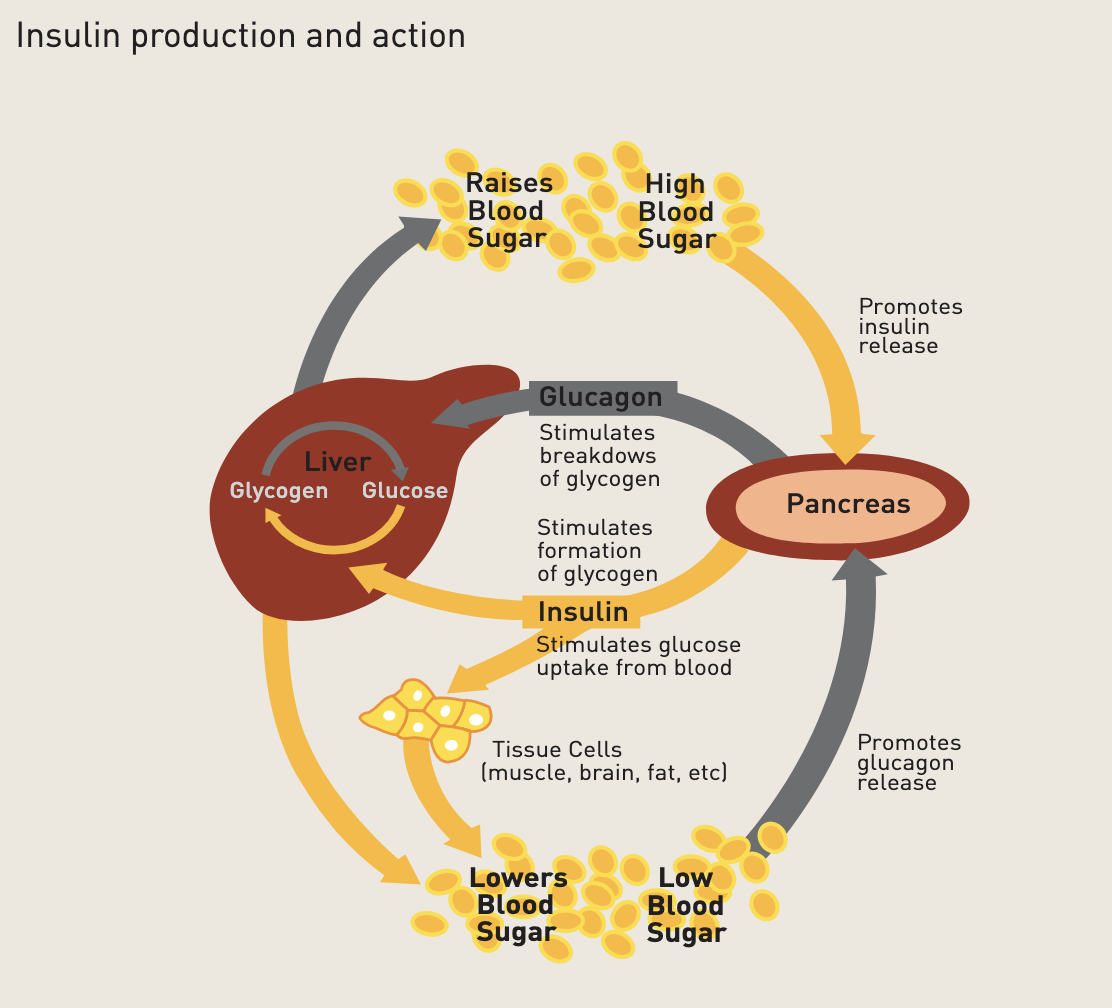
\includegraphics{figures/diabetes_pahtogensis_IDF.png}

}

\caption{Pathogenesis diagram}

}

\end{minipage}%

\end{figure}

The progression from normal glucose metabolism to type 2 diabetes is
characterized by sustained elevations in blood glucose levels, primarily
driven by insulin resistance and followed by a gradual decline in
beta-cell function. Insulin resistance occurs when certain cells, such
as muscle and liver cells, lose their sensitivity to insulin. As a
result, glucose is not effectively taken up by these tissues and remains
in blood circulation. Meanwhile, beta-cell function deteriorates,
leading to a diminished insulin response to glucose intake. Years before
diagnosis, these changes contribute to rising fasting and postprandial
glucose levels. {[}note: read Omar introduction!!!{]}

\begin{figure}

\begin{minipage}[t]{\linewidth}

{\centering 

\raisebox{-\height}{

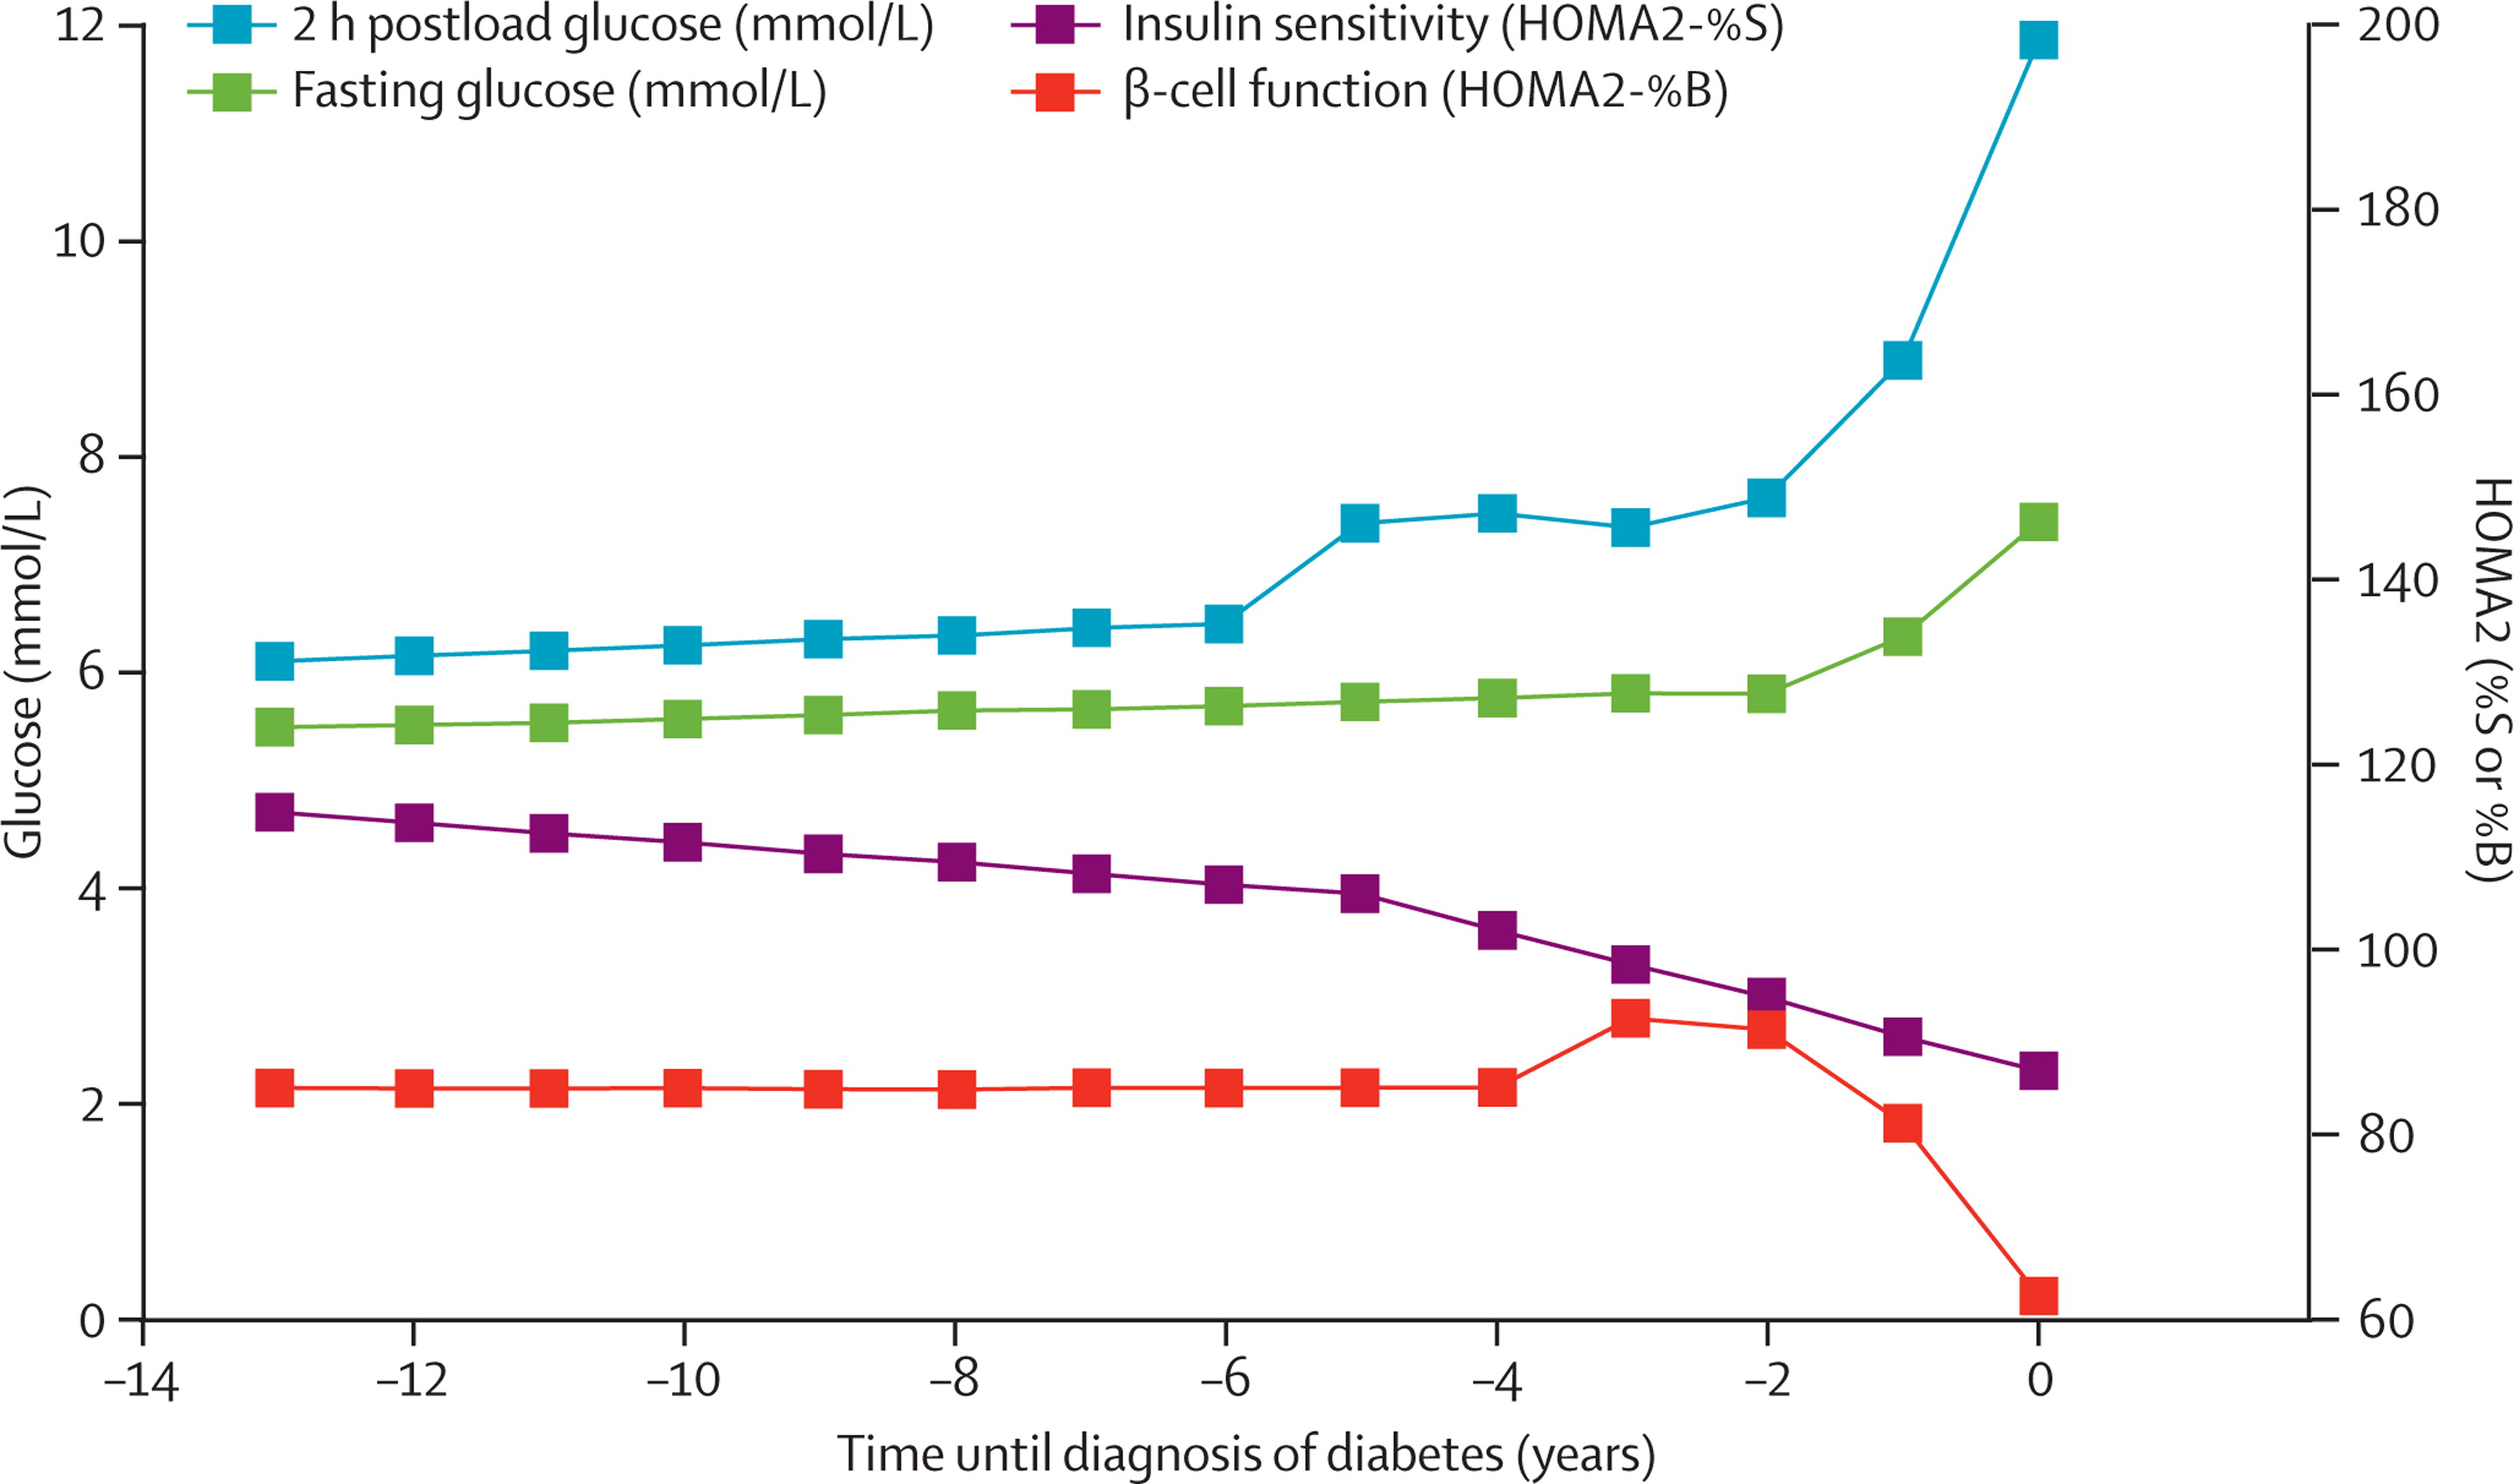
\includegraphics{images/pathogenesis_diabetes.png}

}

\caption{Figure from Tabák AG, Lancet. 2012 Jun 16;379(9833):2279-90}

}

\end{minipage}%

\end{figure}

Diabetes progression is a continuum, with type 2 diabetes defined based
on glucose thresholds associated with an increased risk of
diabetes-specific microvascular complications, particularly retinopathy.
The WHO (2011) and ADA (2015) diagnostic criteria for type 2 diabetes
include fasting plasma glucose ≥7.0 mmol/L, 2-hour plasma glucose ≥11.1
mmol/L during an oral glucose tolerance test, or hemoglobin A1c (HbA1c)
≥6.5\% (48 mmol/mol). However, many other complications of diabetes,
such as macrovascular disease, neuropathy, cancer, and cognitive
impairment, can begin to develop at earlier stages of dysglycemia. This
stage, often referred to as prediabetes or high risk of diabetes, is
defined by fasting plasma glucose levels between 6.1--6.9 mmol/L, 2-hour
plasma glucose levels between 7.8--11.0 mmol/L (WHO criteria), and HbA1c
levels between 5.7--6.4\% (39--47 mmol/mol) (ADA criteria) {[}ref.{]}.

Risk factors for progression to type 2 diabetes and its complications
range from genetic predisposition to lifestyle and socio-environmental
factors. The most common precursor to diabetes is central obesity,
characterized by excess body fat. The accumulation of diabetes risk
factors is linked with a combination of adverse changes in
cardiometabolic markers, including increases in low-density lipoprotein
(LDL) cholesterol, triglycerides, body mass index (BMI), and systolic
blood pressure, along with decreases in high-density lipoprotein (HDL)
cholesterol. {[}Lancet Diabetes Endocrinol 2013; 1: 43--51{]}.

\begin{figure}

\begin{minipage}[t]{\linewidth}

{\centering 

\raisebox{-\height}{

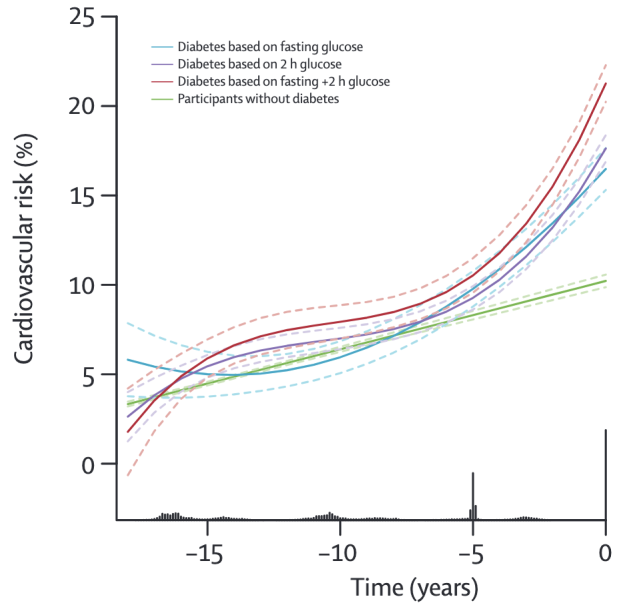
\includegraphics{images/frimingham_risk_before_diabetes.png}

}

\caption{Trajectories of framingham CVD risk score before onset of type
2 diabetes: Lancet Diabetes Endocrinol 2013; 1: 43--51}

}

\end{minipage}%

\end{figure}

Diabetes increases the risk of both microvascular and macrovascular
complications, which are major determinants of the disease's associated
morbidity and mortality. Diabetes and cardiovascular disease share
common risk factors, including lifestyle factors and conventional
clinical markers. As individuals progress toward diabetes, their
cardiovascular risk increases, making them more susceptible to
developing cardiovascular disease (CVD). However, the identification of
preclinical stages and how CVD risk differs among higher-risk
individuals needs further definition. Complications of diabetes has been
included into.

\hypertarget{cardiovascular-disease}{%
\section{Cardiovascular disease}\label{cardiovascular-disease}}

Globally, CVD remains the leading cause of death. However, the main
cause of mortality varies now by country income levels, with cancer
becoming the leading cause in some high-income countries. CVD risk is
primarily attributed to modifiable lifestyle behaviour such as stress,
sedentary behaviour, unhealthy diet, alcohol consumption, and smoking,
as well as socio-environmental factors like socio-economic status and
air pollution (Yusuf et al. 2020). Along the causal pathway to CVD,
these risk factors contribute to comorbidities such as obesity,
diabetes, hypertension, and hypercholesterolemia, further accelerating
overall CVD risk. While risk factors are largely shared across CVD
types, the pathogenesis differs, involving structural, signalling,
inflammatory, and dynamic changes in the cardiovascular system.

\hypertarget{arteriosclerosis}{%
\section{Arteriosclerosis}\label{arteriosclerosis}}

While hard CVD end-points remain the primary focus of CVD prevention
measures, earlier markers of arterial stiffness assess the gradual
vascular pathology and reflect arteriosclerosis, atherosclerosis,
vascular calcification, under vascular aging. Stiffening of the arterial
vasculature increases systolic pressure, reduces coronary perfusion, and
raises the pulsatile load on the microcirculation. Arterial stiffness is
characterized by changes between collagen, elastin, and smooth muscle
cells. With aging, elastic fibers are gradually replaced by collagen
fibers, leading to increased vascular stiffness (Lu et al. 2023). This
process can be accelerated by modifiable risk factors such as smoking,
sedentary behavior, and poor diet, hypertension, dysglycemia and
hyperlipidemia. The progression of arterial stiffness is an early marker
in the trajectory of CVD development, as increased stiffness precedes
rises in blood pressure.

\hypertarget{atherosclerosis}{%
\section{Atherosclerosis}\label{atherosclerosis}}

Atherosclerosis is characterized by plaque build-up in the arteries,
which can develop into a thrombus, leading to artery blockage or
haemorrhage. The underlying process of atherosclerosis is where
cholesterol, fat, and other substances accumulate in the arterial walls,
causing narrowing and reducing blood flow to the heart. When the oxygen
supply to the heart is insufficient, it can result in chest pain
(angina) or, in severe cases, myocardial infarction (heart attack). Over
time, chronic ischemia can lead to structural and functional changes in
the heart, increasing the risk of heart failure and arrhythmia.

\textbf{Myocardial infarction}

Myocardial infarction (MI) occurs due to the rupture of an
atherosclerotic plaque in the coronary arteries, triggering thrombus
formation that blocks blood flow. This leads to oxygen deprivation
(ischemia) and subsequent myocardial injury or necrosis. If untreated,
this process can cause extensive cardiac damage and fatal arrhythmias.
Over the past decades, the incidence rate of MI has decreased in
high-income countries, while improvements in early detection and
treatment (both intravenous and therapeutic) have led to a steep decline
in MI-related mortality. These advancements have also contributed to a
lower prevalence of individuals living with prior MI. In type 2
diabetes, the risk of MI is elevated by 72\%, with an approximately
threefold risk among patients under 60 years compared to age under 60
without type 2 diabetes (Shah et al. 2015). Similar to the general
population, its incidence and fatality have declined in diabetes.

\textbf{Stroke}

Stroke is a cardiovascular disease that can be either ischemic or
hemorrhagic. The majority of strokes are ischemic, caused by an
obstruction in a cerebral artery, often due to an atherosclerotic plaque
or embolism. The second main cause is hemorrhagic stroke, which is
characterized as a hypertensive small-vessel disease, leading to small
lipohyalinotic aneurysms that subsequently rupture, causing
intracerebral bleeding and increased intracranial pressure (Donnan et
al. 2008). Ischemic stroke remains one of the global leading contributor
to mortality and disability (Vos et al. 2020). The trends of incidence,
prevalence and cause-specific mortality of stroke is still elevated and
mostly stagnated but has declined in high income countries (Li et al.
2024). Stroke risk is already elevated at high levels of glucose
(fasting plasma, OGTT, and HbA1c) among people in a pre-diabetic range
where the the risk exceed of 26\% higher risk compared to population
without diabetes {[}Lee et al. (2012){]}(Barr et al. 2007). In type 2
diabetes, the ischemic stroke risk is elevated almost two-fold (Shah et
al. 2015). Hence, the risk of stroke increases with the progression
dysglycemia.

\hypertarget{heart-failure}{%
\section{Heart failure}\label{heart-failure}}

Heart failure gradual develops with age and often. As treatment in
ischemic CVD events has improved survival over the last years, the
incidence and prevalence of heart failure increases. Therefore, early
detection are important as heart failure leads to lower life-expectancy
and quality of life.

Heart failure is a clinical condition characterized by symptoms of
breathlessness, fatigue, and fluid retention, often accompanied by
clinical signs such as pulmonary crepitations, jugular venous elevation,
and peripheral edema. Heart failure can also be defined hemodynamically
as the inability to maintain adequate cardiac output at rest or during
exertion, or the ability to do so only with elevated cardiac filling
pressures. Therefore, it is a complex cardiovascular disease caused by
structural and functional changes in the heart musculature, affecting
systolic and/or diastolic pumping function. Heart failure is generally
classified into two subtypes: heart failure with reduced ejection
fraction (HFrEF) and heart failure with preserved ejection fraction
(HFpEF). Both subtypes involve cardiac remodeling but are defined by
left ventricular ejection fraction (LVEF). HFrEF is characterized by an
LVEF \textless40\%, while HFpEF is identified using various clinical
criteria. HFrEF is often followed by ischemic caused heart failure.

The most common feature of HFpEF is left ventricular diastolic
dysfunction, caused by impaired relaxation and increased stiffness,
leading to elevated left atrial pressure and reduced diastolic reserve
(Normand et al. 2019). Over the past decades, the prevalence of HFpEF
has increased with an aging population and more people living with
pathological conditions such as hypertension, diabetes, and obesity. It
is diagnosed based on abnormal echocardiographic measures of, e.g., left
ventricular hypertrophy, left atrial enlargement, or elevated filling
pressure (Campbell et al. 2024). The diagnosis may seem straightforward,
but it is often challenging in community settings, as patients
frequently present without typical heart failure symptoms (e.g.,
shortness of breath) and are not routinely assessed with biomarkers like
NT-proBNP or brain-neuretic-peptide (BNP). As a result, HFpEF is
commonly underdiagnosed (Campbell et al. 2024).

\hypertarget{cardiovascular-autonomic-dysfunction}{%
\section{Cardiovascular autonomic
dysfunction}\label{cardiovascular-autonomic-dysfunction}}

The cardiovascular system is regulated the autonomic nervous system
which influences heart rate and vasoconstrictuion through
neurotransmitter release by the sympathetic and parasympathetic nerves.
The primary neurotransmitter of the sympathetic nervous system is
noradrenaline, while the parasympathetic nervous system primarily
releases acetylcholine by stimulation through the vagus nerve.
Sympathetic activation increases heart rate and myocardial contractility
by stimulating the sinoatrial (SA) node, atrioventricular (AV) node, and
ventricular myocardium. In contrast, parasympathetic activation
primarily reduces heart rate by directly modulating SA node activity
through vagal stimulation. It also slows AV nodal conduction,
predominantly via the left vagus nerve, thereby prolonging
atrioventricular conduction time. Afferently nerves mainly carry sensory
information (e.g., baroreceptor input from the carotid sinus and aortic
arch) to the brain, which then adjusts efferent autonomic output to
regulate arterial tone. Hence, the autonomic nervous system dynamically
regulates heart rate and blood pressure to maintain homoeostasis in
response to physiological demands, such as rest and physical activity.

{[}insert figure of brain heart and symphathtic nerves{]}

In youth, the autonomic nervous system is highly adaptive and responsive
to living conditions, maintaining autonomic balance. However, with
aging, there is a gradual decline in parasympathetic function and an
increase in sympathetic activity. Additionally, metabolic-related
conditions such as obesity and diabetes have been shown to further
contribute to autonomic dysfunction. Autonomic dysfunction reflects a
stressed cardiometabolic environment, as both dysfunction in lipid and
glucose metabolism are associated with increased sympathetic activity
(Schlaich et al. 2015). This dysfunction may result from cumulative
neural damage mediated by mechanisms such as hyperinsulinemia, insulin
resistance, and elevated levels of adipokines. At the same time,
autonomic dysfunction is known to disrupt lipid and glucose metabolism
(Schlaich et al. 2015). Therefore, the relationship between autonomic
dysfunction and cardiometabolic factors is likely a vicious cycle
(Rinaldi et al. 2023). The consequences can lead to cardiovascular
autonomic dysfunction/neuropathy (CAN), resulting inregulation in heart
rate and vascular dynamics.

Cardiovascular autonomic function is assessed using heart rate
variability (HRV) indices, which measure the variation in successive
normal RR intervals in milliseconds. HRV provides time- and
frequency-domain estimates of the balance between sympathetic and
parasympathetic activity. High HRV reflects an autonomic nervous system
with strong adaptability to the body's demands, whereas low variation
indicates poor adaptation to changing conditions. Most studies have
examined cardiovascular autonomic function using short-term ECG
recordings at rest. However, extended HRV recordings across the
circadian cycle may offer deeper insights into the influence of
lower-frequency variability sources, such as very-low frequency
(0.003--0.04 Hz) and ultra-low frequency (≤0.003 Hz). Hear rate
variability {[}from excercises physiology to psychology, to
cardiovascular research, to diabetes research{]}. Before onset of
diabetes and during progression of diabetes long-term (24-hour HRV) have
shown to be lower compare to those with normal glucose metabolism
{[}Rinaldi et al. (2023){]}(Coopmans et al. 2020). Cardiovascular
autonomic reflex tests (CARTs) are considered the gold standard for
assessing CAN. The diagnosis includes assessing pulse ratio under test
conditions, such as the deep breathing test, the lying-to-standing test,
and the Valsalva maneuver. Both HRV and CARTs have been associated with
cardiovascular disease, heart failure, and all-cause mortality,
primarily in populations with type 2 diabetes or established
cardiovascular disease. However, it remains unclear at which stage in
the progression of diabetes these measures begin to influence the risk
of cardiovascular complications.

\hypertarget{risk-stratification}{%
\section{Risk-stratification}\label{risk-stratification}}

Current cardiopreventive guidelines place strong emphasis on type 2
diabetes. The 2022 ADA/EASD guidelines for the management of
hyperglycemia in type 2 diabetes recommend, cardioprotective medication
GLP-1 receptor agonists and SGLT2-inhibitors as first-line options for
individuals at high cardiovascular risk. Due to their benefits in heart
failure, SGLT2 inhibitors are specifically recommended for patients with
documented HFrEF or HFpEF. High cardiovascular risk is defined as the
presence of at least two risk factors at age \textgreater55 years, such
as obesity, hypertension, smoking, dyslipidemia, or albuminuria.
However, no additional preclinical markers are recommended to identify
individuals at higher CVD risk. Despite their increased risk of
cardiovascular complications, individuals at high risk of developing
diabetes remain outside structured treatment options, even though
diabetes risk and cardiometabolic markers can be successfully modified
through lifestyle interventions and medication such as GLP-1 analogoues
{[}{``Reduction in the Incidence of Type 2 Diabetes with Lifestyle
Intervention or Metformin''} (2002){]}(Kahn et al. 2024). During the
progression and after the onset of type 2 diabetes, preclinical stages
may manifest with markers of higher cardiovascular risk, underscoring
the potential for risk stratification. Risk stratification is the
process of classifying individuals based on risk scores, biomarker
levels, omic data (metabolomic, proteomics, and genomic) or preclinical
conditions. This approach aids in subtyping patients for prognostic or
diagnostic purposes, identifying subgroups that require further
evaluation, intensified treatment, or lifestyle modifications.

\begin{figure}

\begin{minipage}[t]{\linewidth}

{\centering 

\raisebox{-\height}{

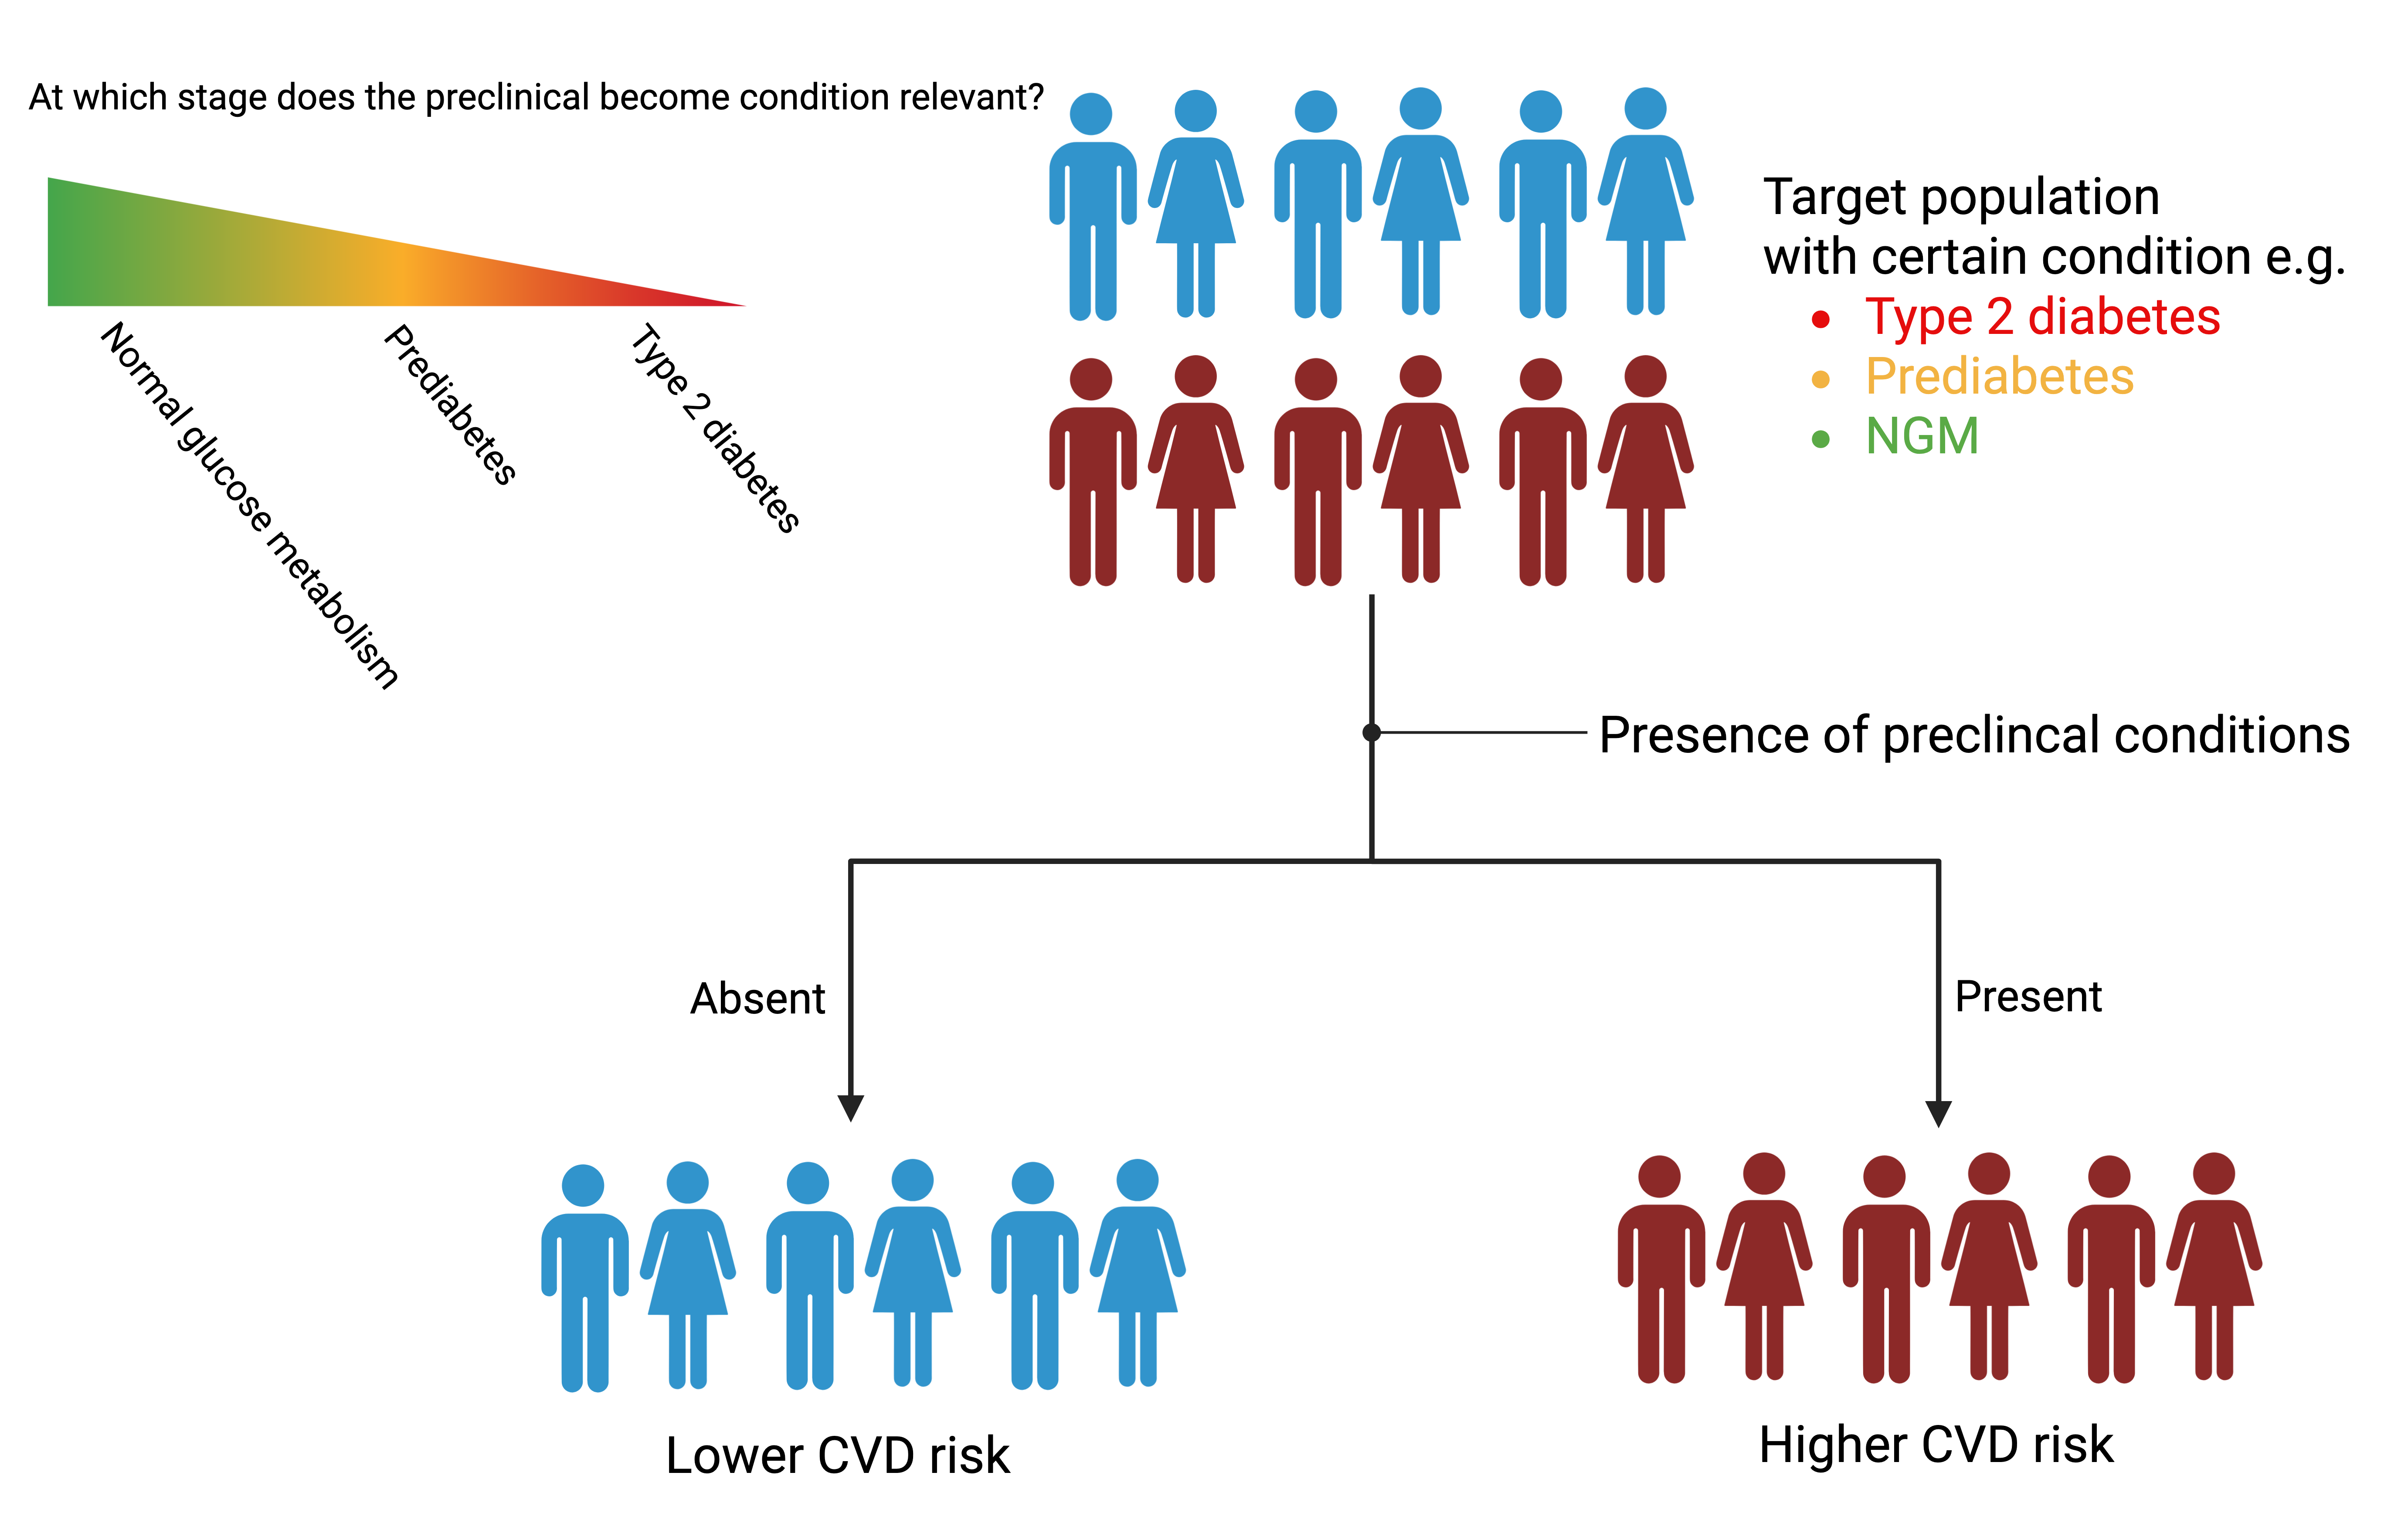
\includegraphics{images/risk_stratification.png}

}

\caption{Risk-stratification based on preclinical disease}

}

\end{minipage}%

\end{figure}

Cardiovascular autonomic dysfunction despite it's relationship with
cardiovascular complication has not been defined into clinical practice.
Larger epidemiological cohort studies encompassing various stages of
diabetes risk, from normal glucose metabolism to prediabetes, onset of
type 2 diabetes, and longer term progression of type 2 diabetes, serve
as valuable resources for identifying risk-stratification opportunities.
Epidemiological studies provide a broad representation of the target
population, allowing understand the relationship between cardiovascular
autonomic dysfunction and cardiovascular complications. They also have
potential to determine when, along the trajectory of diabetes
progression and duration, autonomic function are meaningful for
cardiovascular risk-stratification.

\hypertarget{aetiological-research}{%
\section{Aetiological research}\label{aetiological-research}}

Aetiology identifies the causes and contributing factors of disease,
forming the foundation for understanding its development and underlying
mechanisms. Bradford Hill established nine criteria to assess the
strength of causality: Strength (effect size), Consistency
(reproducibility), Specificity, Temporality, Biological Gradient
(dose--response relationship), Plausibility, Coherence, Experiment, and
Analogy. Although these criteria are somewhat controversial, as they are
not strictly procedural for epidemiological research, they serve as
guiding principles for evaluating causality in research findings. In
cardiovascular disease, socio-environmental influences and personal
health behaviours play a crucial role in overall health and are
considered the outer contributing layer to biological mechanism. The
inner layer focuses on biological causal processes, where the connection
between these contributing factors and individual predisposition to
cardiovascular disease remains a key question in understanding the
underlying pathological mechanisms.

\begin{figure}

\begin{minipage}[t]{\linewidth}

{\centering 

\raisebox{-\height}{

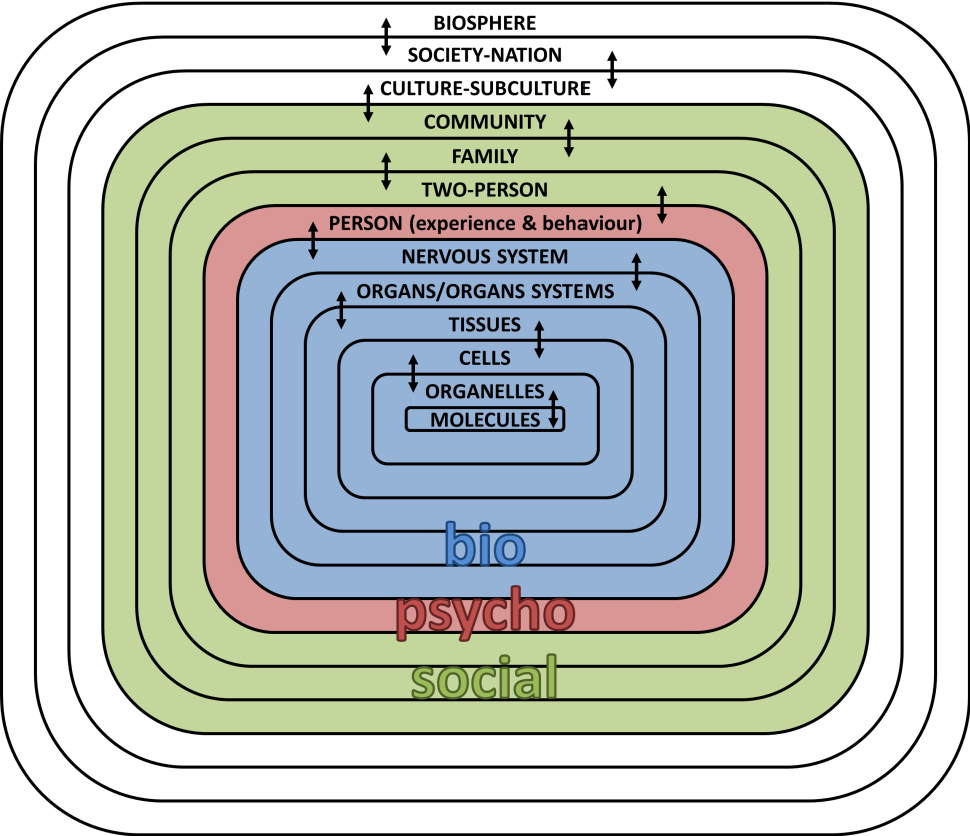
\includegraphics{images/physcosocial_model.png}

}

\caption{Biopsychosocial model}

}

\end{minipage}%

\end{figure}

Cardiovascular autonomic dysfunction is linked to CVD and all-cause
mortality. However, many questions remain regarding the underlying
causal mechanisms. Furthermore, as dysglycemia is known to be a primary
driver of autonomic dysfunction (Jeffrey J. Goldberger et al. 2019), the
questions is to which extent it modulates the relationship between
cardiovascular autonomic dysfunction and CVD? This relationship remains
unclear, highlighting the need for a deeper understanding of this
interplay in target populations representing different stages of glucose
metabolism.

\bookmarksetup{startatroot}

\hypertarget{aim-and-hypothesis}{%
\chapter{Aim and hypothesis}\label{aim-and-hypothesis}}

The overall aim of this PhD is to understand how cardiovascular
autonomic dysfunction/neuropathy (CAN) affects cardiovascular disease
risk (i.e.~heart failure, stroke, myocardial infarction) and specific
subclinical markers of CVD: carotid-femoral pulse wave velocity and
carotid artery distensibility in populations covering the whole glycemic
continuum, from healthy glucose metabolism to type 2 diabetes.

Study I: Quantify the cross-sectional association between 24-hour HRV
and subclinical markers of cardiovascular complications: carotid-femoral
pulse wave velocity and carotid artery distensibility, in a participants
with normoglycemia, prediabetes or type 2 diabetes.

Study II: Quantify the longitudinal association of week-long and hourly
HRV with incidence ischemic-CVD, heart failure, and all-cause mortality
in a population with high-risk of diabetes.

Study III: Quantify the cross-sectional association between CAN and
heart failure. Heart failure will be defined by clinical measures
i.e.~N-terminal-pro-BNP (Pro-BNP), electrocardiogram (ECG), and New York
Heart Association (NYHA) scores among individuals with type 2 diabetes.

The hypotheses of this dissertation are:

CAN and autonomic dysfunction is associated with CVD and acts as an
early risk factor for heart failure and other cardiovascular
complications, including stroke, and myocardial infarction in patients
with prediabetes and/or T2D. In addition autonomic dysfunction is
associated with higher levels of carotid-femoral pulse wave velocity and
carotid artery distensibility.

\bookmarksetup{startatroot}

\hypertarget{materials-and-methods}{%
\chapter{Materials and methods}\label{materials-and-methods}}

\hypertarget{overview-of-the-studies}{%
\section{Overview of the studies}\label{overview-of-the-studies}}

\begin{longtable}[]{@{}
  >{\raggedright\arraybackslash}p{(\columnwidth - 6\tabcolsep) * \real{0.2083}}
  >{\raggedright\arraybackslash}p{(\columnwidth - 6\tabcolsep) * \real{0.2639}}
  >{\raggedright\arraybackslash}p{(\columnwidth - 6\tabcolsep) * \real{0.3056}}
  >{\raggedright\arraybackslash}p{(\columnwidth - 6\tabcolsep) * \real{0.2222}}@{}}
\caption{Table 1: Overview of studies}\tabularnewline
\toprule\noalign{}
\begin{minipage}[b]{\linewidth}\raggedright
\end{minipage} & \begin{minipage}[b]{\linewidth}\raggedright
Study I
\end{minipage} & \begin{minipage}[b]{\linewidth}\raggedright
Study II
\end{minipage} & \begin{minipage}[b]{\linewidth}\raggedright
Study III
\end{minipage} \\
\midrule\noalign{}
\endfirsthead
\toprule\noalign{}
\begin{minipage}[b]{\linewidth}\raggedright
\end{minipage} & \begin{minipage}[b]{\linewidth}\raggedright
Study I
\end{minipage} & \begin{minipage}[b]{\linewidth}\raggedright
Study II
\end{minipage} & \begin{minipage}[b]{\linewidth}\raggedright
Study III
\end{minipage} \\
\midrule\noalign{}
\endhead
\bottomrule\noalign{}
\endlastfoot
Title & Cardiovascular autonomic dysfunction is linked with arterial
stiffness across glucose metabolism: The Maastricht Study &
Cardiovascular autonomic dysfunction precedes cardiovascular disease and
all-cause mortality: 11-year follow-up in the ADDITION-PRO study &
Cardiovascular autonomic neuropathy and subclinical heart failure in
type 2 diabetes: The CANCAN study \\
Design & Aetiological cross-sectional study & Aetiological prospective
cohort study & Descriptive cross-sectional study \\
Cohort & Maastricht study & ADDITION-PRO & CANCAN \\
Study population & 3673 people with normal glucose metabolism,
prediabetes, and type 2 diabetes & 2082 people with high risk of
diabetes & 173 patients with type 2 diabetes visiting outpatients
clinics \\
Data sources & Population-based cohort from The Maastricht Study in the
Netherlands & Cohort study of selected people based on having high risk
of diabetes & Clinical cohort study \\
Determinant & 24-hour HRV & Week-long and hourly HRV & Cardiovascular
autonomic reflex test \\
Primary outcome & Arterial stiffness & Major adverse cardiovascular
events, heart failure, and all-cause mortality & NT-proBNP \\
Statistical analysis & Linear regression & Poisson regression & Logistic
regression \\
Missing data & Complete case analysis & Multiple imputation of chained
equations for confounders & Multiple imputation of chained equations for
CART and confounders \\
\end{longtable}

\hypertarget{study-population}{%
\subsection{Study population}\label{study-population}}

\begin{figure}

\begin{minipage}[t]{\linewidth}

{\centering 

\raisebox{-\height}{

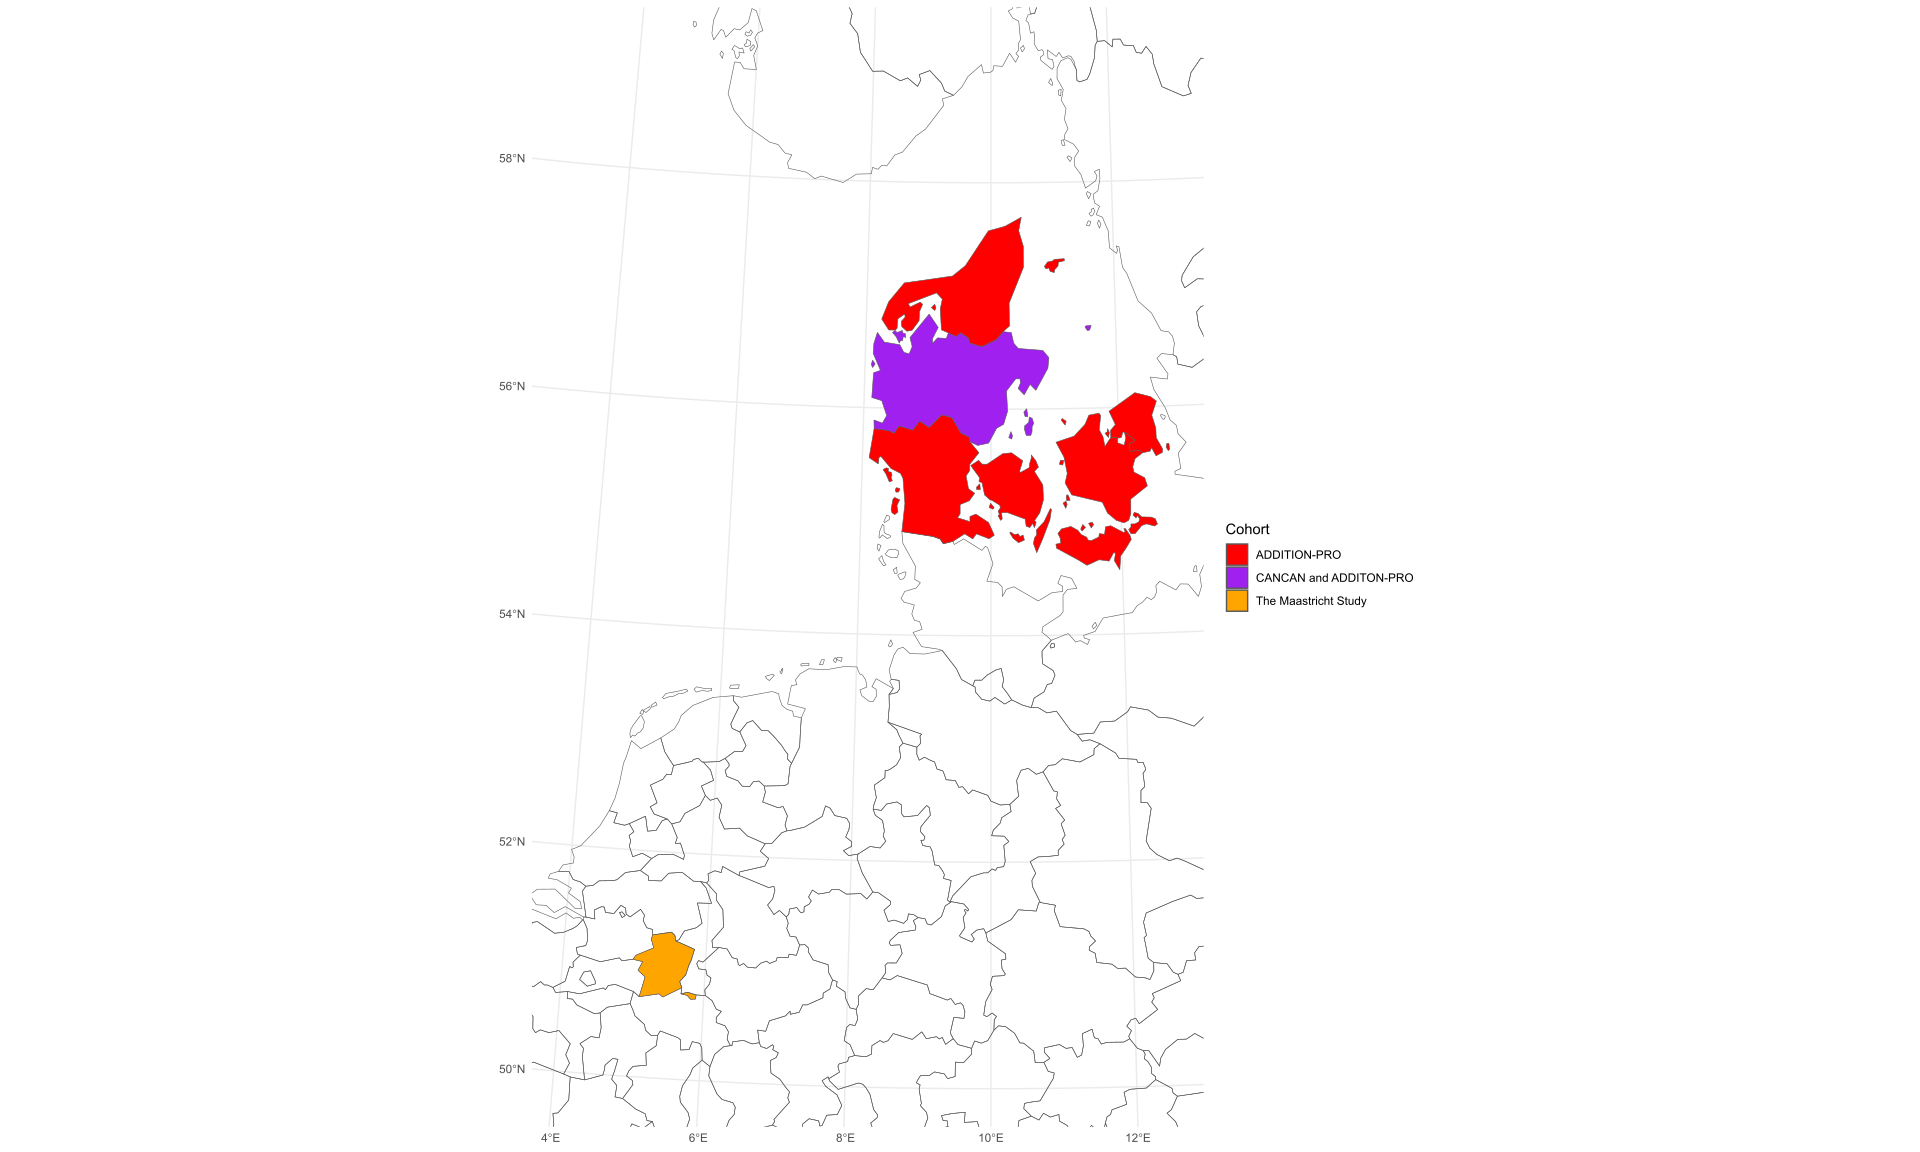
\includegraphics{images/cohort_map.png}

}

\caption{Study populations}

}

\end{minipage}%

\end{figure}

\hypertarget{study-i---the-maastricht-study}{%
\subsubsection{Study I - The Maastricht
Study}\label{study-i---the-maastricht-study}}

The Maastricht Study is a prospective observational population-based
study of the general population in the southern part of the Netherlands.
The study emphasized the recruitment of people with type 2 diabetes,
through the regional Diabetes Patient Registry, to extensively phenotype
individuals with type 2 diabetes and those in intermediate stages of the
disease. The eligibility criteria included an age range of 40--70 years.
Participants were recruited through mass media campaigns and mailings
from municipal registries (Gemeentelijke Basis Administratie; GBA). In
the analysis of Study I, the study among 7449 population included
participants with measurements of 24-hour HRV and at least one measure
of arterial stiffness (carotid-femoral pulse wave velocity or carotid
artery distensibility), both of which were completed within a
three-month period between November 2010 and December 2020. The study
has been approved by the institutional medical ethics committee
(NL31329.068.10) and the Minister of Health, Welfare and Sports of the
Netherlands (Permit 131088-105234-PG). All participants gave written
informed consent.

\hypertarget{study-ii---addition-pro}{%
\subsubsection{Study II - ADDITION-PRO}\label{study-ii---addition-pro}}

The ADDITION-PRO study is a prospective population-based cohort nested
within the Danish arm of the ADDITION-Europe study, originally designed
as a stepwise screening program for type 2 diabetes in general practice.
ADDITION-PRO aims to investigate early markers of cardiovascular disease
(CVD) and metabolic dysfunction in individuals in different tiers of
diabetes risk.

The ADDITION-Europe screening program identified a large number of
individuals with impaired fasting glucose (IFG), impaired glucose
tolerance (IGT), and normoglycemia despite having risk factors for
diabetes and CVD. Participants for ADDITION-PRO were recruited from the
original ADDITION-DK screening cohort, which included individuals from
190 general practices across Denmark. The recruitment strategy focused
on individuals at high risk of diabetes withou type 2 diabetes,
identified through a stepwise screening program that incorporated the
Danish diabetes risk score from the Inter99. This assessment, conducted
between 2001 and 2006, considered factors such as age, sex, history of
gestational diabetes, family history of diabetes, known hypertension,
BMI, and physical activity. High risk individuals was further screen for
type 2 diabetes by blood measurement including HbA1c, random blood
glucose, FPG, and OGTT, were identified patients were invited to the
ADDITION-trail. High risk individuals without type 2 diabetes was
further considered in a sampling fram for ADDITION-PRO.

Between 2009 and 2011, a follow-up health examination was conducted at
four ADDITION-DK study centers to establish a longitudinal cohort.
Eligible participants were those still alive, residing near the research
centers (Steno Diabetes Center Copenhagen, Aarhus University Hospital,
Holstebro Hospital, and the Hospital of South West Jutland, Esbjerg),
and who had not withdrawn consent. Eligibility criteria included
individuals aged 40--70 years who had previously undergone diabetes
screening in ADDITION-DK. Exclusion criteria included pregnancy,
psychological or psychiatric disorder preventing informed consent, and
life-limiting conditions. One key feature of the data collection was the
precise measurement of physical activity and energy expenditure using
ActiHeart, which recorded acceleration and heart rate over a week. We
included participants with a least 48-hour recording for our first
analysis, and then include those participants with hourly measures of
physical acceleration during the hourly HRV recording for th second
analysis. We also excluded participant with prior CVD ten years before
inclusion.

The population were disease history and follow-up in the unique register
system of Denmark, which allows linkage of health records using the
personal Civil Registration Number assigned to all citizens. The
following national registries were accessed to collect information on
incident CVD and mortality, medication use, and healthcare utilization:
the National Patient Registry (hospital admissions and outpatient
contacts), the National Health Service Registry (general practice
visits), the Medical Prescription Registry, the Diabetes Registry, and
the Cause of Death Registry.

\hypertarget{study-iii---cancan}{%
\subsubsection{Study III - CANCAN}\label{study-iii---cancan}}

The CANCAN Study was an observational pilot study conducted at two
hospital outpatient clinics in Viborg Regional Hospital and Regional
Hospital Gødstrup. It aimed to implement a screening protocol for
identifying high-risk individuals using CAN assessments, continuous
glucose monitoring, and heart failure indicators. All measures were part
of routine clinical care for type 2 diabetes in Central Denmark. We
included 200 adults (\textgreater18 years) with type 2 diabetes for over
one year. Exclusion criteria were recent laser-treated eye disease (≤3
months), pregnancy, lactation, life-threatening illness, or cognitive
impairment preventing consent. Participants were identified via
electronic records and informed about the study by their doctor during
telephone call. Those interested attended a dedicated meeting before
their annual diabetes exam, where study details were discussed.
Recruitment took place from 2021 to 2024. In study III, participants
without a valid NT-proBNP measurement were excluded.

\hypertarget{study-variables}{%
\section{Study variables}\label{study-variables}}

\hypertarget{measures-for-cardiovascular-autonomic-dysfunction-neuropathy}{%
\subsection{Measures for cardiovascular autonomic dysfunction/
neuropathy}\label{measures-for-cardiovascular-autonomic-dysfunction-neuropathy}}

\textbf{Heart rate variability}

\begin{figure}

\begin{minipage}[t]{\linewidth}

{\centering 

\raisebox{-\height}{

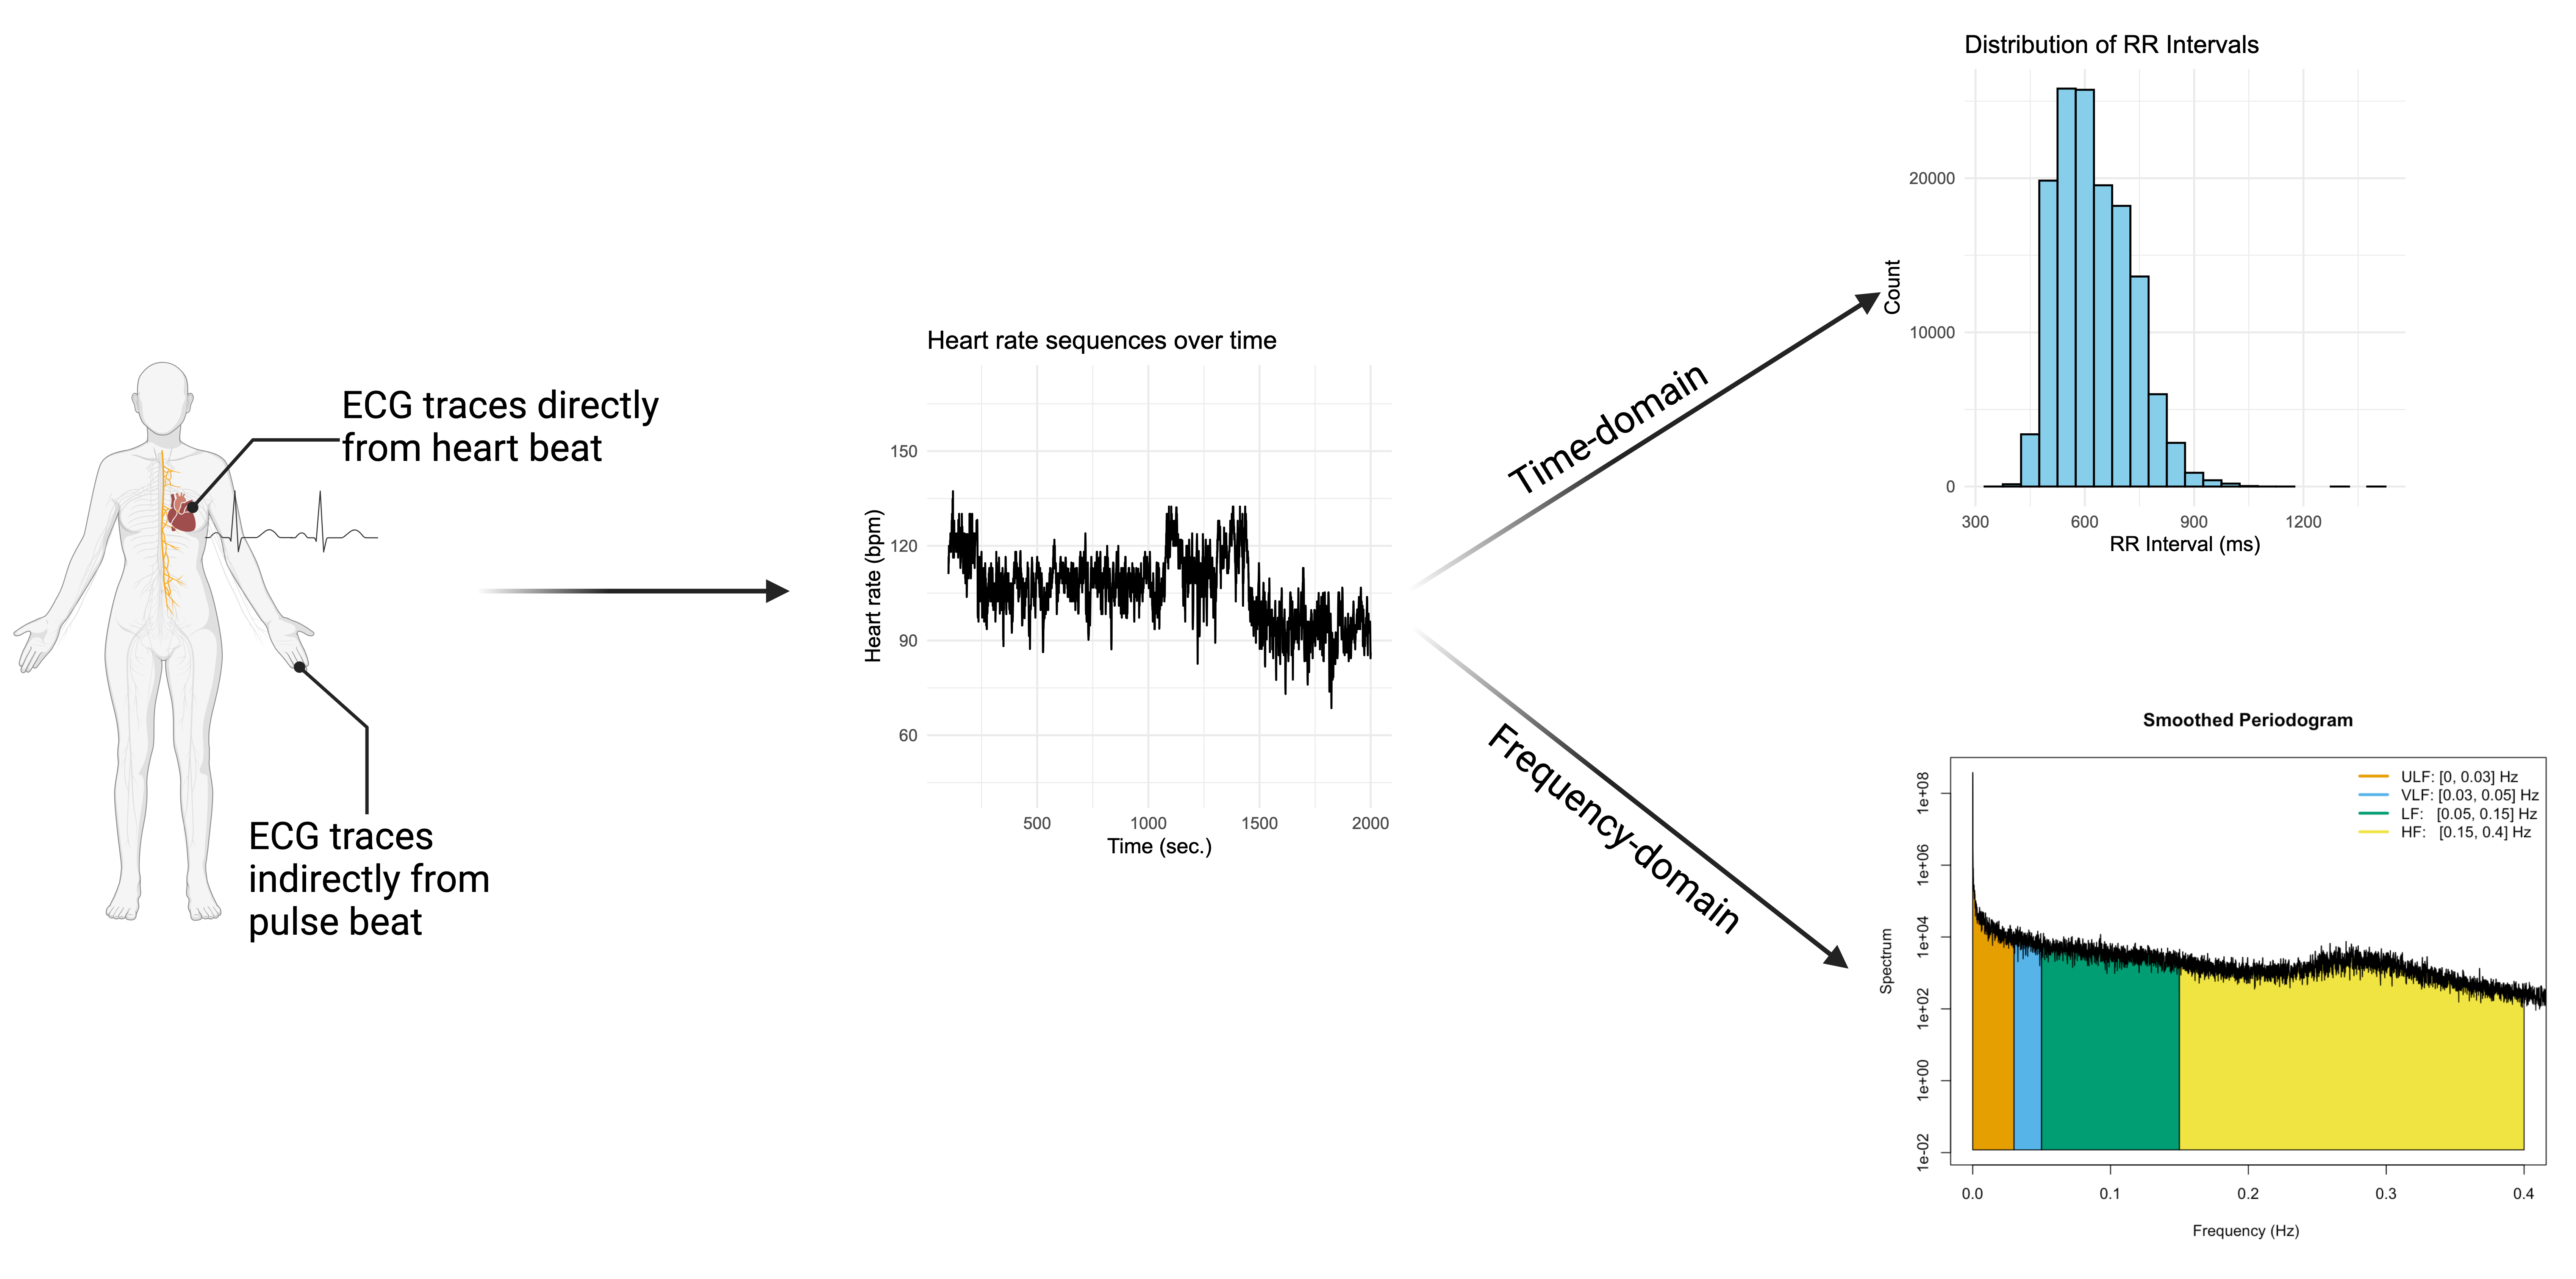
\includegraphics{images/measurements_hrv.png}

}

\caption{Heart rate variability}

}

\end{minipage}%

\end{figure}

In study I-III a device was used to capturing the distance between each
heartbeat defined as RR intervals from electrocardiogram traces either
directly from heart-beat traces or indirectly from pulse traces. From
this a sequence of successive heart beat intervals is extracted to
calculate HRV. The pool of hearbeat data, we extrapolated time-domain
and frequency-domain HRV indices. In study III, we used the ratio in
pulse rate in test under different conditions lying-to-stading, in-
expiration, and valsalva maneuvre.

\emph{Time-domain indices}

Time-domain measures of HRV are based on the statistical distribution of
normal-to-normal (NN) intervals. These include the standard deviation
(SD) of NN intervals, the variation in successive NN intervals, and the
proportion of successive intervals that differ by more than 50 ms.
Description of time-domain indices are summarized in box 1.

\begin{longtable}[]{@{}
  >{\raggedright\arraybackslash}p{(\columnwidth - 2\tabcolsep) * \real{0.5000}}
  >{\raggedright\arraybackslash}p{(\columnwidth - 2\tabcolsep) * \real{0.5000}}@{}}
\caption{Box 1: Time-domain HRV indices}\tabularnewline
\toprule\noalign{}
\begin{minipage}[b]{\linewidth}\raggedright
Time-domain HRV
\end{minipage} & \begin{minipage}[b]{\linewidth}\raggedright
Description
\end{minipage} \\
\midrule\noalign{}
\endfirsthead
\toprule\noalign{}
\begin{minipage}[b]{\linewidth}\raggedright
Time-domain HRV
\end{minipage} & \begin{minipage}[b]{\linewidth}\raggedright
Description
\end{minipage} \\
\midrule\noalign{}
\endhead
\bottomrule\noalign{}
\endlastfoot
\textbf{Standard deviation of NN heart beat intervals (SDNN, in ms)} &
Reflects overall HRV and total autonomic nervous system activity over
the recording period. \\
\textbf{SD of the averages of NN intervals in 5-minute segments
throughout the recording (SDANN, in ms)} & Measures long-term HRV
variations, primarily reflecting circadian and autonomic
fluctuations. \\
\textbf{Mean of the SDs of all NN intervals for all 5-minute segments
(SDNN index, in ms)} & Estimates short-term HRV fluctuations and vagal
tone by averaging segmental variations. \\
\textbf{NN50 count divided by the total number of all NN intervals
(pNN50, percentage)} & Represents the proportion of successive NN
intervals differing by more than 50 ms, indicating vagal activity. \\
\textbf{Square root of the mean of the sum of squares of differences
between adjacent NN intervals (RMSSD, in ms)} & Reflects short-term HRV,
mainly parasympathetic (vagal) activity. \\
\end{longtable}

\emph{Frequency-domain indices}

Frequency-domain HRV indices are derived from sequences of NN intervals
transformed into the spectral domain using Fourier transformation. These
indices quantify heart rate oscillations over different timescales.
Short-term variations, such as respiratory sinus arrhythmia, reflect
rapid autonomic changes, while longer oscillations capture autonomic
responses to posture changes, circadian rhythms, or other physiological
processes. Description of frequency-domain indices are summarized in box
2.

\begin{longtable}[]{@{}
  >{\raggedright\arraybackslash}p{(\columnwidth - 2\tabcolsep) * \real{0.3472}}
  >{\raggedright\arraybackslash}p{(\columnwidth - 2\tabcolsep) * \real{0.6528}}@{}}
\caption{Box 2: Frequency-domain HRV indices}\tabularnewline
\toprule\noalign{}
\begin{minipage}[b]{\linewidth}\raggedright
Frequency domain HRV
\end{minipage} & \begin{minipage}[b]{\linewidth}\raggedright
Description
\end{minipage} \\
\midrule\noalign{}
\endfirsthead
\toprule\noalign{}
\begin{minipage}[b]{\linewidth}\raggedright
Frequency domain HRV
\end{minipage} & \begin{minipage}[b]{\linewidth}\raggedright
Description
\end{minipage} \\
\midrule\noalign{}
\endhead
\bottomrule\noalign{}
\endlastfoot
\textbf{Variance of all NN intervals ≤ 0.4 Hz, total power (TP, in ms²)}
& Represents overall HRV, reflecting both short- and long-term autonomic
regulation. \\
\textbf{Ultralow-frequency range (ULF, in ms² ≤ 0.003 Hz)} & Captures
very long-term oscillations, influenced by circadian rhythms,
metabolism, and thermoregulation. \\
\textbf{Very-low-frequency range (VLF, in ms²; 0.003--0.04 Hz)} &
Associated with sympathetic activity, inflammation, and hormonal
regulation. \\
\textbf{Low-frequency range (LF, in ms²; 0.04--0.15 Hz)} & Reflects a
mix of sympathetic and parasympathetic activity, often linked to blood
pressure regulation and baroreflex sensitivity. \\
\textbf{High-frequency range (HF, in ms²; 0.15--0.4 Hz)} & Represents
parasympathetic (vagal) modulation of heart rate, closely related to
respiratory sinus arrhythmia. \\
\end{longtable}

\textbf{Holter recordings in study I}

All ECG recordings were obtained using a 12-lead Holter system
(Fysiologic ECG Services, Amsterdam, the Netherlands) over 24 hours, as
previously described. Participants were instructed to follow their
regular daily activities but avoid showering during the recording. The
ECG data were processed using proprietary Holter Analysis Software
(Fysiologic ECG Services), where artefacts and ectopic beats were
excluded through automated processing and manual validation. A minimum
recording duration of 18 hours was required for further analysis.
Inter-beat intervals between consecutive sinus beats were provided in
milliseconds (ms). Time-domain HRV indices were calculated, including
SDNN, SDANN, RMSSD, SDNN index, and pNN50. Frequency-domain measures
were derived using Fast Fourier Transform, including TP, ULF, VLF, LF,
and HF. Outliers were removed. HRV indices were standardised by their
mean and SD, and composite Z-scores were computed for time and
frequency-domain measures, respectively. This selection of indices
covers the main sources of HRV variance.

\textbf{ActiHeart heart rate and physical activity in study II}

Heart rate was measured using a combined accelerometer and heart rate
monitor (ActiHeart, CamNTech, Cambridge, UK), recording uniaxial
acceleration and heart rate. The data collection and processing methods
have been described previously. Mean heart rates were recorded in
30-second epochs, and HRV was derived as the variation between
consecutive normal heartbeats on the ECG. HRV calculations were
performed using the RHRV package (version 4.2.7) in R, including SDNN,
SDANN, SDNN index, TINN, and mean HR (mHR). We tested our approach on a
dataset with full access to all interbeat intervals to validate our
algorithm(J. Schaarup 2024). These indices have shown high validity for
global HRV assessment in 24-hour recordings. HRV indices were calculated
by week, 24-hour cycle, and hour of the day, with hourly values averaged
across recording days.

\textbf{Vagus device for cardiovascular autonomic reflex test in study
III}

CAN was diagnosed using cardiovascular autonomic reflex tests (CARTs),
the gold standard for CAN assessment. R-R intervals were derived from an
ECG signal using the Vagus™ device (Medicus Engineering, Aarhus,
Denmark). Three standardized CARTs were performed: lying-to-standing,
deep breathing, and the Valsalva manoeuvre, following a standardized
protocol between 8:00 a.m. and 2:00 p.m. after 10 minutes of supine
rest. Smoking and caffeine intake were prohibited two hours before
testing. Each test was conducted once by trained examiners.

Manifest CAN was defined as two or more abnormal CARTs using
age-specific cut-off values (ref.). The Vagus™ device's accuracy has
been validated against FDA standards and stationary devices, showing
moderate to high reproducibility (ref.).

\begin{figure}

\begin{minipage}[t]{\linewidth}

{\centering 

\raisebox{-\height}{

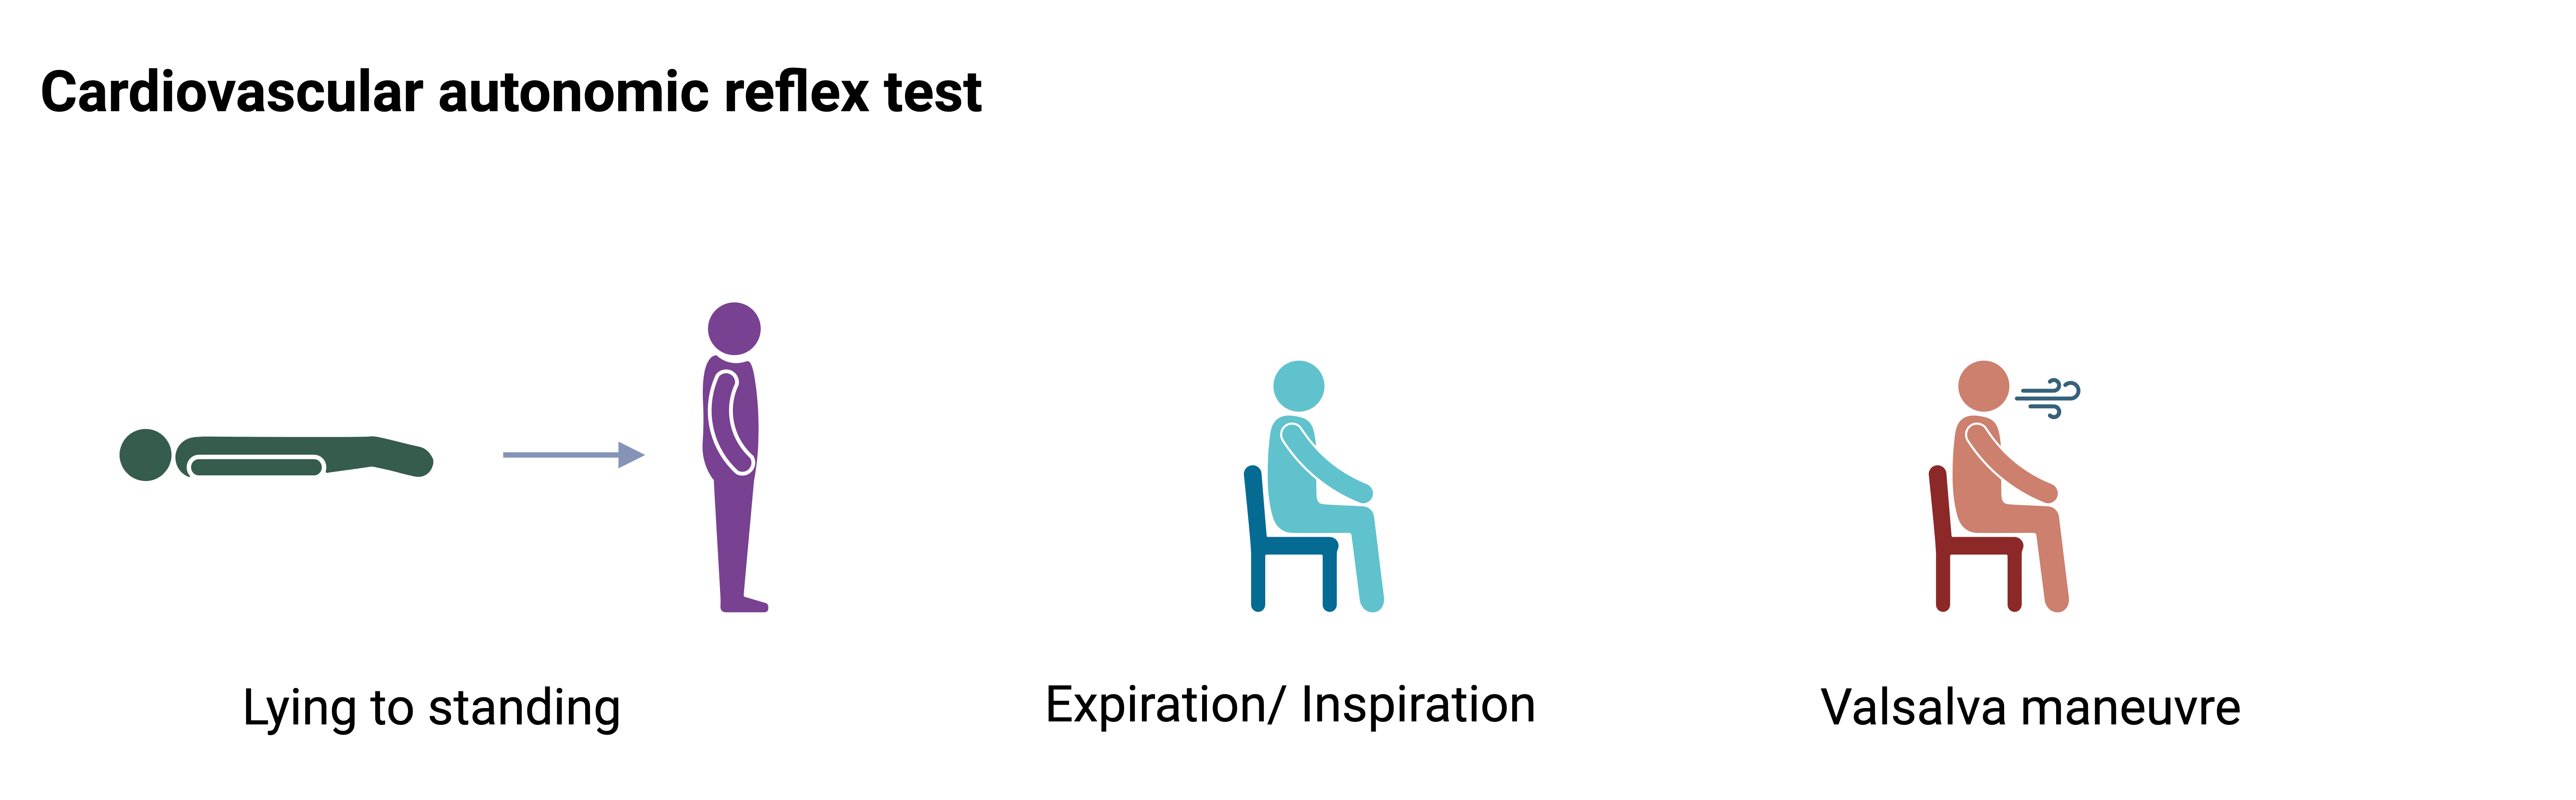
\includegraphics{images/cart.png}

}

\caption{CART}

}

\end{minipage}%

\end{figure}

HRV was derived from all CARTs using autoregressive spectral analysis.
Time domain measures included SDNN and RMSSD, while frequency domain
measures included LF, HF, and total power. Orthostatic hypertension was
defined as a sustained drop in systolic blood pressure of ≥20 mmHg or
diastolic blood pressure of ≥10 mmHg within three minutes of standing
(ref.).

\hypertarget{confounders-and-variables-for-instrumental-bias}{%
\subsection{Confounders and variables for instrumental
bias}\label{confounders-and-variables-for-instrumental-bias}}

\textbf{Lifestyle} Smoking status was

\textbf{Clinical markers}

\textbf{Medication}

\hypertarget{outcomes}{%
\section{Outcomes}\label{outcomes}}

\hypertarget{arterial-stiffness}{%
\subsection{Arterial stiffness}\label{arterial-stiffness}}

\textbf{Pulse wave velocity}

Arterial stiffness can be characterized by measuring arteriosclerosis
and atherosclerosis properties of the arteries. The stiffness of
different trees of the vascular musculature can assessed both locally
and dynamically. Aortic and carotid stiffness were assessed as markers
of arterial stiffness, following previously described procedures. Aortic
stiffness was measured by carotid-femoral pulse wave velocity (PWV)
using applanation tonometry (SphygmoCor, Atcor Medical, Sydney,
Australia), with the median of at least three consecutive recordings
included in the analysis.

\textbf{Carotid artery distensibility}

Carotid stiffness was assessed by the carotid artery distensibility
coefficient (CD), based on ultrasound imaging of the left common carotid
artery using a 7.5 MHz linear probe (MyLab 70, Esaote Europe,
Maastricht, the Netherlands). CD was calculated as ΔD/braPP, where ΔD
represents carotid distension and braPP is brachial pulse pressure. Mean
heart rate and mean arterial pressure (MAP) were recorded every five
minutes using an oscillometer device (Accutorr Plus, Datascope,
Montvale, NJ, USA).

{[}insert figure of PWV and CD{]}

\hypertarget{biomarker}{%
\subsection{Biomarker}\label{biomarker}}

N-terminal prohormone of brain natriuretic peptide (NT-proBNP) is a
neuretic peptide that can be used to detect patients with heart failure
and the progression. It derives from B-type natriuretisk peptid (BNP)
which is a cardial neurohormon, that is syntezied and secreted as
response to streched cariomycytes and cardiac volume overload. After
secretion, proBNP is cleaved, releasing the active hormone BNP along
with the remaining N-terminal fragment, known as NT-proBNP. In study
III, blood sample were taken at study cite. Description of the NT-proBNP
analysis of plasma samples is described in supplementary material
{[}ref.{]}.

\hypertarget{cardiovascular-events}{%
\subsection{Cardiovascular events}\label{cardiovascular-events}}

Information on CVD events and mortality was obtained from the Danish
National Patient Registers until 2021. ICD-10 codes for stroke,
myocardial infarction, cardiovascular death, cardiovascular
revascularization, and heart failure.

\textbf{Ischemic heart disease}

We defined three-point major adverse cardiovascular events (MACE) as
myocardial infarction, stroke, cardiovascular revascularization, and
cardiovascular death.

\textbf{Heart failure}

We defined heart failure by all diagnosis codes, including ``DI50,'' for
hospitalisation with heart failure.

\hypertarget{statistical-methods}{%
\section{Statistical Methods}\label{statistical-methods}}

\hypertarget{cross-sectional-analysis}{%
\subsubsection{Cross-sectional
analysis}\label{cross-sectional-analysis}}

In study I, we used multiple linear regression to investigate
associations between week-long HRV and arterial stiffness. Model 1
adjusted for age, sex, education, glucose metabolism status, and mean
arterial pressure (MAP) to account for the oversampling of individuals
with type 2 diabetes and potential instrumental bias of arterial
pressure flow. Model 2 included additional adjustments for smoking
behavior, alcohol consumption, physical activity, body mass index,
HbA1c, triglycerides, total-to-HDL cholesterol ratio, and medication
use. Arterial stiffness measures were log-transformed to ensure normally
distributed residuals and back-transformed into percentage change
estimates. We add interaction sex to oberve if the association differed
between sex. We performed sensitivity analyses excluding individuals on
antihypertensive treatment or glucose-lowering medication. In study III,
we applied logistic regression models to investigate the association
between CAN and heart failure, using NT-proBNP as the primary outcome.
We adjusted for age, sex, and diabetes duration, smoking behavior,
alcohol consumption, body mass index, HbA1c, triglycerides, total
cholesterol, and antihypertensive medication, eGFR and prior CVD. We
performed sensitivity analyses excluded participants with beta-blocker
treatment or prior CVD.

\hypertarget{effect-modification}{%
\paragraph{Effect modification}\label{effect-modification}}

In study I, we hypothesize that the association between 24-hour and
arterial stiffness was stronger in strata of progression of diabetes
(normal glucose metabolism, prediabetes, type 2 diabetes). We therefore
first stratified by diabetes status to observe the size of the
association across strata. We then combine all groups and include an
interaction term between HRV and diabetes status. We did subsidiary
analysis to check if the effect was modified by dysglycemia by
stratifying HbA1c and fasting plasma glucose into deciles.

\hypertarget{time-to-event-analysis}{%
\subsubsection{Time-to-event analysis}\label{time-to-event-analysis}}

In study II, we used Poisson regression models to quantify the
associations between HRV and cardiovascular events, as follow-up data
were undisturbed over time and to avoid assumptions of proportional
hazards(2012). Week-long HRV was modelled using splines with knots at
predefined percentiles to assess non-linear associations. Hourly HRV was
analysed separately for each hour to observe if the association of HRV
had diurnal variation. Both HRV and mHR were standardized by their mean
and standard deviation to ensure comparability. Based on assumptions
about potential confounding pathways summarized in directed acyclic
graphs (DAG), we fitted two models: Model 1 adjusted for age and sex,
while Model 2 further adjusted for education, smoking, alcohol
consumption, physical activity (physical activity energy expenditure
(PAEE) calculated from Recent Physical Activity Questionnaire RPAQ),
body mass index, total cholesterol, and HbA1c. Additional analyses were
performed with HRV pre-adjusted for concurrent heart rate and physical
acceleration to account the influence of these factors. Missing
covariates were handled using multiple imputation.

\hypertarget{multiple-imputed-by-chained-equations}{%
\subsection{Multiple imputed by chained
equations}\label{multiple-imputed-by-chained-equations}}

Multiple Imputation by Chained Equations (MICE) is a method for handling
missing data in datasets. This procedure imputes missing values through
an iterative series of predictive models, generating plausible estimates
while preserving the relationships within the data. To avoid one
imputation for missing value could give the value the same confidence as
the a non-missing value, we followed Rubins Rule. Rubin's rules in MICE
combine results from multiple imputed datasets by pooling estimates of
interest (e.g., means or regression coefficients) using their within-
and between-imputation variances. Thus, we ensure valid statistical
inferences by accounting for the uncertainty introduced by missing data.

In study II, we imputed confounders to include as many participants and
avoid excluding population with our without cardiovascular or mortality
events. We imputed dataset 10 times. In study III, we imputed missing
CART, as a proportion of participants had non-valid test due to
insufficient air in the valsalva manuevre, unstable heart beats or data
error. All available variables of biochemical measures, diagnosis,
medication and cause of non-valid CART was used to impute CART using
predictive mean matching.

\hypertarget{instrumental-bias}{%
\subsection{Instrumental bias}\label{instrumental-bias}}

In study I-III we are investigating the body properties by dynamic
measures and biomarkers to quantify autonomic function, arterial
stiffness, and cardiac function. Other conditions may affect the
properties we are attempting to measure, and thus are causing
instrumental bias.

\emph{Vascular Stiffness}

In Study I, we used measurements of arterial stiffness using cf-PWV and
carotid distensibilty. Both measures are influenced by arterial pressure
at the time of examination. Arterial pressure affects the propagation of
the pressure wave through the aorta (cf-PWV) and the expansion and
contraction of the carotid artery (carotid distensibilty.) {[}ref.{]}.
To account for this, we adjusted for mean arterial pressure in our
models.

\emph{Cardiovascular autonomic function}

In Study II, we assessed cardiovascular autonomic function using
week-long HRV recordings and hourly HRV measurements. Studies have
highlighted that HRV is dependent on heart rate, and low HRV may simply
reflect a higher resting heart rate (rHR). To adjust for this without
overcorrecting for a collinear variable, we pre-adjusted HRV by
regressing rHR on HRV, extracting the residuals, and using these as the
pre-adjusted determinant. For hourly HRV, variability in heart rate may
be influenced by changes in physical activity, creating a risk that HRV
serves as a proxy for movement rather than autonomic function. To
address this, we applied a similar pre-adjustment approach by regressing
concurrent heart rate and physical acceleration to account for physical
activity.

\emph{Biomarker of Heart Failure}

In Study III, kidney function and overweight are know to influence
NT-proBNP levels beyond heart failure. We adjusted the model to account
for the blurred effect of eGFR on NT-proBNP levels in the analysis.

\bookmarksetup{startatroot}

\hypertarget{results-xxxxx-current-xxxxx}{%
\chapter{Results (xx,xxx current:
xx,xxx)}\label{results-xxxxx-current-xxxxx}}

In this section, I will summarize study population characteristics and
findings from analysis.

\hypertarget{study-i}{%
\section{Study I}\label{study-i}}

\hypertarget{descriptive}{%
\subsection{Descriptive}\label{descriptive}}

In The Maastricht Study, {[}10,000 participated by Date{]}, of those
1316 reported prior CVD. Participants who had valid 24-hour HRV measured
was 4379 and of those 3673 had a valid measurement of either CD or PWV.
Study population included 3673 participants. Further characteristic are
described in the study I manuscript {[}Table 1{]} {[}refeernce to study
I{]}.

\begin{table}
\centering
\begin{tabular}{l|l|l|l}
\hline
**Characteristic** & **Normal glucose metabolism**  
N = 2,389 & **Prediabetes**  
N = 538 & **Type 2 Diabetes**  
N = 746\\
\hline
Sex &  &  & \\
\hline
Men & 1,028 (43\%) & 280 (52\%) & 481 (64\%)\\
\hline
Women & 1,361 (57\%) & 258 (48\%) & 265 (36\%)\\
\hline
Age (years) & 58 (51, 64) & 62 (57, 68) & 63 (57, 68)\\
\hline
Total physical activity (hours/week) & 13 (9, 19) & 13 (9, 19) & 12 (7, 17)\\
\hline
Moderate to vigorous physical activity (hours/week) & 5.3 (3.0, 8.3) & 4.5 (2.3, 7.5) & 3.8 (1.5, 6.8)\\
\hline
BMI (kg/m²) & 25.0 (22.9, 27.4) & 27.2 (24.9, 30.1) & 28.8 (26.0, 31.7)\\
\hline
Waist (cm) & 89 (81, 97) & 98 (90, 105) & 103 (96, 112)\\
\hline
HbA1c (\%) & 5.35 (5.17, 5.63) & 5.63 (5.35, 5.90) & 6.54 (6.08, 7.09)\\
\hline
Fasting plasma glucose (mmol/L) & 5.10 (4.80, 5.40) & 5.90 (5.40, 6.30) & 7.40 (6.60, 8.50)\\
\hline
LDL (mmol/L) & 3.20 (2.70, 3.90) & 3.30 (2.60, 4.00) & 2.40 (1.80, 3.10)\\
\hline
HDL (mmol/L) & 1.60 (1.30, 2.00) & 1.40 (1.20, 1.80) & 1.30 (1.00, 1.50)\\
\hline
Total cholesterol (mmol/L) & 5.50 (4.80, 6.20) & 5.50 (4.80, 6.30) & 4.50 (3.90, 5.20)\\
\hline
Triglycerides (mmol/L) & 1.05 (0.80, 1.45) & 1.39 (1.03, 1.90) & 1.51 (1.08, 2.14)\\
\hline
Duration of type-2 diabetes (only for diagnosed participants) & NA (NA, NA) & NA (NA, NA) & 3 (0, 9)\\
\hline
Mean IBI (ms) & 838 (775, 907) & 815 (760, 897) & 806 (744, 889)\\
\hline
SDNN (ms) & 138 (117, 164) & 127 (106, 152) & 116 (96, 139)\\
\hline
RMSSD (ms) & 26 (21, 34) & 24 (19, 33) & 22 (17, 31)\\
\hline
SDANN (ms) & 125 (103, 149) & 113 (92, 139) & 103 (84, 127)\\
\hline
SDNNi (ms) & 55 (46, 65) & 50 (41, 60) & 44 (36, 54)\\
\hline
pNN50 (\%) & 7 (3, 13) & 5 (2, 10) & 4 (2, 9)\\
\hline
TP (ms²) & 12,596 (8,880, 17,498) & 10,615 (7,134, 15,374) & 8,880 (6,064, 12,722)\\
\hline
ULF (ms²) & 10,771 (7,392, 15,142) & 8,948 (5,852, 13,374) & 7,524 (5,036, 11,001)\\
\hline
VLF (ms²) & 1,198 (833, 1,692) & 1,015 (685, 1,478) & 816 (541, 1,267)\\
\hline
LF (ms²) & 421 (257, 651) & 328 (200, 540) & 261 (154, 422)\\
\hline
HF (ms²) & 94 (57, 158) & 78 (47, 138) & 63 (36, 117)\\
\hline
Systolic blood pressure (mmHg) & 123 (114, 133) & 129 (122, 140) & 130 (122, 139)\\
\hline
Diastolic blood pressure (mmHg) & 75 (71, 80) & 78 (73, 83) & 76 (72, 81)\\
\hline
Mean arterial pressure (mmHg) & 95 (88, 102) & 99 (93, 107) & 98 (92, 105)\\
\hline
Carotid artery distensibility (10-3/kPa) & 15.0 (11.8, 18.8) & 13.5 (10.4, 16.9) & 12.5 (9.9, 16.0)\\
\hline
Carotid-femoral pulse wave velocity (m/s) & 8.08 (7.28, 9.16) & 8.96 (7.84, 10.32) & 9.36 (8.16, 10.80)\\
\hline
N\_HT & 833 (35\%) & 317 (59\%) & 590 (79\%)\\
\hline
Antihypertensive medication & 431 (18\%) & 199 (37\%) & 478 (64\%)\\
\hline
med\_HT\_beta & 149 (6.2\%) & 77 (14\%) & 195 (26\%)\\
\hline
Lipid-lowering medication & 280 (12\%) & 141 (26\%) & 484 (65\%)\\
\hline
\end{tabular}
\end{table}

\hypertarget{hour-hrv-and-arterial-stiffness}{%
\subsection{24-hour HRV and arterial
stiffness}\label{hour-hrv-and-arterial-stiffness}}

\textbf{Time-domain HRV}

In the fully adjusted model 2, PWV was 2.8\% (CI: 2.1; 3.4) lower, while
CD was 3.3\% (CI: 1.5; 5.1) higher per SD increase in HRV time-domain
Z-score. Among the time-domain indices, SDNN, SDNNi, and SDANN showed
the strongest associations, with cf-PWV being lower by 2.5\% (CI: 2.0;
3.1), 2.5\% (CI: 1.9; 3.4), and 2.2\% (CI: 1.7; 2.7), respectively.
Conversely, CD was higher by 3.2\% (CI: 1.7; 4.7), 3.0 \% (CI: 1.4;
4.6), and 2.8\% (CI: 1.3; 4.3), respectively. RMSSD and pNN50 showed a
weaker association with cf-PWV (-1.1\% {[}CI: -1.4; -0.4{]}, and -1.1
{[}-1.7; -0.6{]}), while no evidence for an association was found with
CD.

\textbf{Frequency-domain HRV}

In the fully adjusted model 2, PWV was 2.8\% (CI: 2.1; 3.5) lower, while
CD was 3.2\% (CI: 1.3; 5.1) higher per SD increase in HRV
frequency-domain Z-score. Among the frequency-domain indices, total
power, VLF, and ULF showed the strongest associations, with cf-PWV being
lower by 2.2\% (CI: 1.7; 2.8 ), 2.4\% (CI: 1.9; 4.0), and 2.1\% (CI:
1.5; 2.6), respectively. Conversely, CD was higher by 2.7\% (CI: 1.2;
4.2), 2.4\% (CI: 0.9; 4.1), and 2.6\% (CI: 1.1; 4.1), respectively. HF
showed a weaker association with cf-PWV (-0.9\% {[}CI: -1.4; -0.4{]}),
while no evidence for an association was found with CD. Mean interbeat
interval was associated with 2.4 \% (CI: 1.8; 2.9) lower cf-PWV and
4.5\% (3.1; 6.1) higher CD.

\hypertarget{effect-modification-of-diabetes-status}{%
\subsection{Effect modification of diabetes
status}\label{effect-modification-of-diabetes-status}}

The study population represented diabetes risk of normal glucose
metabolism (65\%), prediabetes (15\%), and type 2 diabetes (20\%). The
median (IQR) cf-PWV (aortic stiffness) increased with diabetes status:
NGM: 8.08 m/s (7.28, 9.16), prediabetes: 8.96 m/s (7.84, 10.32), and
type 2 diabetes: 9.36 m/s (8.16, 10.80). CD (carotid stiffness)
decreased: NGM: 15.0 (11.8, 18.8), prediabetes: 13.5 (10.4, 16.9), and
type 2 diabetes: 12.5 (9.9, 16.0) × 10⁻³/kPa. SDNN (ms) was highest in
NGM and decreased with worsening glucose metabolism: NGM: 138ms (117,
164), prediabetes: 127ms (106, 152), and type 2 diabetes: 116ms (96,
139).

The association between HRV time-domain Z-scores and cf-PWV and CD was
significantly modified by prediabetes (PWV: -4.9 {[}CI: -6.523;
-3.243{]} \(^{interaction(*) ^{p-value< 0.01}}\) CD: 8.0 {[}CI:3.8;
12.5{]}\(^{*^{p-value< 0.01}}\)) but not by type 2 diabetes (PWV: -3.5
\% {[}CI: -4.8; -2.1){]} \(^{*^{p-value< 0.1}}\) CD: 4.8 \% {[}CI:1.3;
8.4{]}\(^{*^{p-value< 0.1}}\)). For the indices SDNN and SDANN, the
association with both cf-PWV and CD was significantly modified by both
prediabetes and type 2 diabetes.

The association between HRV frequency-domain Z-score and cf-PWV was
significantly modified from normal glucose metabolism by prediabetes
(-5.7 \%{[}CI:-7.4; -3.9{]}\(^{*^{p-value< 0.01}}\)) and type 2 diabetes
(-3.9 \%{[}CI:-5.4; -2.3{]}\(^{*^{p-value< 0.05}}\)) while CD was only
modified by prediabetes (8.3 \%{[}CI:3.6;
13.2{]}\(^{*^{p-value< 0.01}}\)) but not by type 2 diabetes (5.3
\%{[}CI:1.4; 9.4{]}\(^{*^{p-value< 0.1}}\)). For the indices total power
and ULF, the association with both cf-PWV and CD was significantly
modified by both prediabetes and type 2 diabetes. Mean inter beat
interval association with cf-PWV or CD was not significantly modified by
diabetes status.

Prototypical individuals representing diabetes risk from normal glucose
metabolism, to prediabetes to type 2 diabetes {[}edit text from
manuscript about comparison between 95th percentile and 5th
percentile{]} showed to have xx\% higher PWV and xx\% lowed CD. Among
people with prediabetes and type 2 diabetes the difference was xx\%
higher PWV and xx\% lowed CD and xx\% higher PWV and xx\% lowed CD,
respectively.

{[}Different risk \% higher by diabetes status (NGT, prediabetes,
T2D){]}

{[}FPG and Hba1c values and the interaction and the magnitude of the
association between HR and AS{]}

\hypertarget{study-ii}{%
\section{Study II}\label{study-ii}}

\hypertarget{descriptive-1}{%
\subsection{Descriptive}\label{descriptive-1}}

In ADDITION-PRO population consisted of 1,627 participant with a least
48-hour HRV measures, while 1,432 had all hour represented with hourly
HRV and physical acceleration. The study population included different
tiers of diabetes risk: 154 individuals at low risk (9\%), 889 at high
risk (51\%), 314 with impaired fasting glucose (IFG) (18\%), 226 with
impaired glucose tolerance (IGT) (13\%), and 161 with both IFG and IGT
(9\%). We splitted SDNN into categories by very-low (SDNN\textless{} 100
ms), low (SDNN 100-120 ms), middle (SDNN 121-140 ms), high (SDNN 141-160
ms) and very-high (SDNN \textgreater160 ms).

{[}Higher age (68 years (6.3)), BMI (28.2 kg/m\^{}2 (4.7)), HbA1c (5.9
\% (0.6)), triglyceride (1.4 (0.8)), and higher proportion of men
(63\%), and users of anti-hypertensive medication (60\%) was observed
among participants who experienced MACE or heart failure compared to
participants without any CVD{]} replace with SDNN distribution{]} .

\hypertarget{week-long-hrv-and-mace-heart-failure-and-all-cause-mortality.}{%
\subsection{Week-long HRV and MACE, heart failure, and all-cause
mortality.}\label{week-long-hrv-and-mace-heart-failure-and-all-cause-mortality.}}

The mean week-long SDNN was 139.0 (32.3) ms, and the mean heart rate was
73.5 (9.1) bpm. In the fully adjusted model, SDNN per SD was associated
with a lower incidence rate ratio (IRR) for MACE 0.82 (CI: 0.69; 0.97),
heart failure 0.76 (CI: 0.58; 0.99), and mortality rate ratio of 0.79
(CI: 0.66; 0.94). When we included knots in the model, the trends
indicated that the risk increased when SDNN fell below 120-110 ms
(approximately below 20th percentile), suggesting a potential cut-off
point for higher risk. We therefore calculate incidence rate with SDNN
levels at 100 ms, 120ms, and 160 ms, respectively, and plotted by a
function of age.

{[}Incedence rate curves{]}

\hypertarget{hourly-hrv-and-mace-heart-failure-and-all-cause-mortality.}{%
\subsection{Hourly HRV and MACE, heart failure, and all-cause
mortality.}\label{hourly-hrv-and-mace-heart-failure-and-all-cause-mortality.}}

From the hourly recordings, we observed a clear periodicity in SDNN,
mean heart rate (HR), sleep patterns, and physical acceleration. SDNN
increased from 5--6 AM, peaking at 8--9 AM {[}mean (SD){]}, followed by
a gradual decline, reaching its lowest point around 1 AM the next day
{[}mean SDNN (SD){]}. A similar circadian pattern was observed in heart
rate, though its peak occurred two hour later at 10--11 AM. After
peaking, heart rate remained stable throughout the afternoon before
gradually decreasing.

{[}include results from hourly results{]}

\hypertarget{study-iii}{%
\section{Study III}\label{study-iii}}

\hypertarget{descriptive-2}{%
\subsection{Descriptive}\label{descriptive-2}}

In study III, 179 participants with type 2 had measures of NT-proBNP and
performed the CART test. CAN was present in 30\% (n = 54) of
participants (36\% among those with valid CAN measurements). Meanwhile,
24\% (n = 43) were unable to complete the CART assessment adequately,
primarily due to irregular heart rhythms (n = 8) or insufficient air
pressure during the Valsalva manoeuvre (n = 21). Compare to those
without CAN, the participants with CAN were more women (41 \% vs 33 \%),
were more sedentary (45\% vs 36\%), had a higher proportion with prior
major CVD (41\% vs 20\%) and declined eGFR (\textless{} 60) (36\% vs
22\%), higher levels of triglyceride (median 2.05 mmol/L vs 1.95 mmol/
L), were slightly older (median 62 years vs 61 years), had longer
duration of type 2 diabetes (median 19 years vs 15 years), and higher
use SGTL2-inhibitors (65\% vs 60\%) but lower use of GLP-1 RA (63\% vs
70\%). No other difference in clinical characteristic was observed.

\hypertarget{relationship-between-can-and-elevated-nt-probnp}{%
\subsection{Relationship between CAN and elevated
NT-proBNP}\label{relationship-between-can-and-elevated-nt-probnp}}

A greater proportion of individuals with CAN exhibited elevated
NT-proBNP levels (\textgreater125 pg/ml) (51.9\%, n=52/78) compared to
those without CAN (23.2\%, n=26/112). The fully adjusted odds ratio (OR)
for elevated NT-proBNP in individuals with CAN was 5.69 (95\% CI: 1.95,
18.49) relative to those without CAN. Among the cardiovascular autonomic
reflex tests (CART), the Valsalva maneuver demonstrated the strongest
association with NT-proBNP (OR 9.00, 95\% CI: 2.88, 33.09; n=51/75),
followed by deep breathing (OR 3.30, 95\% CI: 1.17, 9.77; n=33/133) and
orthostatic hypertension (OR 4.04, 95\% CI: 1.27, 13.77; n=24/146). No
significant association was identified for the lying-to-standing test
(OR 0.80, 95\% CI: 0.32, 1.97; n=54/108). After imputing missing CART
data, the OR for CAN in relation to elevated NT-proBNP declined to 2.94
(95\% CI: 1.37, 6.56). Sensitivity analyses, which excluded participants
using beta-blockers or those with a history of CVD, resulted in a
smaller sample size and wider confidence intervals, though the overall
association remained unchanged.

\bookmarksetup{startatroot}

\hypertarget{discussion-17280-current-14479}{%
\chapter{Discussion (17,280 current:
14,479)}\label{discussion-17280-current-14479}}

\hypertarget{strength-and-limitation}{%
\section{Strength and limitation}\label{strength-and-limitation}}

\hypertarget{study-design}{%
\subsection{Study design}\label{study-design}}

\emph{Cross-sectional design}

Studies I and III are based on cross-sectional data, with exposure and
outcome measured within a three-month period. The main limitation of
this design is that it does not allow us to determine whether the
exposure led to the outcome or vice versa. As a result, we cannot
establish temporarily or confirm whether changes in the outcome were
caused by the exposure. However, based on prior evidence, we assume the
direction of the studies based on physiological knowledge and in vivo
studies. In Study I, we based our direction of the association based on
longitudinal association based on data from Whitehall II study, showing
steeper decrease in short-term HRV are associated with subsequent higher
levels of cf-PWV. Moreover, {[}insert in vivo studies{]}. In Study II,
we attempted to mimic temporarily by glucose metabolism, in individuals
with type 2 diabetes and without known type 2 diabetes, instead of time,
which shows deterioration of glucose metabolism increases the size of
the association. The strength of study I, is that sample size is large,
making our results more generalisable to wider populations across
statuses of glucose metabolism.

In study III, our design are more focused on the clinical diagnosis of
CAN and presence of heart failure. This the question are more focused on
clinical utilization of CAN in detecting type 2 diabetes patients who
early progress towards heart failure, and thus the aetiological question
remain for other study design. Indeed, whether cardiac function
progressively worsens due to the etiological mechanisms of CAN remains
to be fully established. If confirmed, this would underscore the
relevance of CAN as a preclinical marker for early progression to heart
failure, one that may be effective to target in efforts to prevent or
delay the development of overt heart failure.

\emph{Longitudinal design}

A major strength of study II is its longitudinal design, where HRV was
measured at baseline and outcomes were captured prospectively through
national registries. This temporal structure ensures that the exposure
(HRV) clearly preceded the outcome, reducing the risk of reverse
causation. Although repeated measurements of HRV over time would provide
more detailed insights into autonomic function dynamics, the prospective
design still allows for stronger inference of directionality than
cross-sectional studies. Furthermore, the use of high-quality registry
data for outcome ascertainment ensures complete follow-up and minimizes
loss to follow-up bias.

Based on our studies, we demonstrate first steps in relationship between
cardiovascular autonomic function, measured by, heart rate variability
or CART, we can only establish an association and cannot conclude with
certainty that improvements in HRV measures lead to a reduction in
cardiovascular risk. Therefore, we cannot ascertain causal effect based
on our findings, and more causal focused methods are needed. Mendelian
randomization, which uses genetic instruments for exposure, could help
address this causal question. Furthermore, structured mediation analysis
involving modification, e.g.~by medication or lifestyle, would improve
HRV or CART leads to reduction in cardiovascular risk, using data from
intervention studies.

\hypertarget{intern-validity}{%
\subsection{Intern validity}\label{intern-validity}}

In this project, we aimed to assess cardiovascular autonomic function
both in free-living conditions and in response to standardized test
procedures during clinical visits. Additionally, we used dynamic
measurements to evaluate arterial stiffness locally and by velocity and
biomarker assessments to determine the presence of heart failure. In
this section, I will discuss the validity of 24-hour, week-long, and
hourly HRV measurements, as well as the standardized tests of CAN.
Furthermore, I will address the validity of the included outcomes. I
will as well discuss using the strength and limitation of using MACE as
an time to event outcome.

\hypertarget{measures-of-autonomic-dysfunction}{%
\subsubsection{Measures of autonomic
dysfunction}\label{measures-of-autonomic-dysfunction}}

HRV has been applied across several research domains. For example, in
psychology as a marker of mental stress, in exercise physiology as an
indicator of recovery, in cardiovascular research as a marker of
autonomic dysfunction related to cardiac complications, and in diabetes
research as a marker of autonomic neuropathy. In the context of this
project, which focuses on long-term HRV in diabetes and cardiovascular
research, it is important to acknowledge that the autonomic nervous
function we aim to assess, may also be influenced by behavioural factors
such as physical activity, sleep, meal timing, emotions, smoking,
caffeine intake, alcohol consumption, use of medication, and prior
cardiovascular complications. Therefore, reduced long-term HRV cannot be
interpreted solely as a marker of autonomic function. Factors such as
sleep, stress, meals, and physical activity can influence HRV both
during recordings potentially masking or mimicking underlying
physiological dysfunction. Moreover, HRV is also influenced by lifestyle
patterns over time, making it sensitive not only to acute behaviours but
also to long-term habits that affect autonomic balance. In study II, we
observed that the lower ranges of HRV had both lower habitual physical
acitivty and lower VO\textsubscript{2} max, suggesting that lower HRV
reflects more sedentary lifestyle and lower cardiorespiratory fitness.

Although this poses a limitation in physiological research attempting to
disentangle the causal pathways between autonomic dysfunction and
cardiovascular disease, it simultaneously highlights a potential target
for intervention, given that low HRV may be indicative of adverse
lifestyle patterns. For instance, behavioural patterns such as disrupted
sleep or irregular meal timing may influence circadian fluctuations in
HRV. Evidence from studies on night-shift workers suggests that meal
timing affects HRV, with daytime meals leading to higher HRV during
night hours (Chellappa et al. 2025). Thus, although long-term HRV may
lack the precision to disentangle sympathetic and parasympathetic
activity due to overlapping behavioural and physiological influences, it
may be a valuable tool for assessing autonomic responses in free-living
conditions and informing lifestyle-based strategies to improve
cardiovascular health.

When using long-term HRV recordings, careful consideration is needed to
determine how best to utilize the data in relation to the specific
research objectives. In diabetes and cardiovascular research, 24-hour
HRV measures of high-frequency indices such as RMSSD and pNN50 are more
sensitive to behavioral influences and therefore have not consistently
shown strong associations with cardiovascular or metabolic outcomes,
especially when compared to measures based on total variability.
However, when HRV is analyzed in shorter segments (e.g., hourly or in
5-minute intervals), high-frequency measures like RMSSD, pNN50, and HF
appear to offer new insights into autonomic function and its relevance
in diabetes and cardiovascular disease. {[}find reference!!!{]}. SDANN
and SDNNi aim to reduce the impact of short-term variability, such as
that caused by physical activity, by calculating either the standard
deviation of 5-minute segment mean IBI (SDANN) or the mean of standard
deviations across 5-minute segments (SDNNi). This helps smooth out
transient fluctuations and better capture long-term autonomic
modulation.

In study I and II, we strived to account for habitual physical activity,
while in study II, we also accounted hourly HRV for physical
acceleration during the recording to test the influence. However,
further studies are need to understand how lifestyle patterns affect the
long-term recording the subsequent day, to understand the behavioural
component in long-term HRV. In study I and II, we also excluded
participants to ensure that in order to keep aetiological order between
autonomic dysfunction and the outcome of cardiovascular complication,

*Anti-hypertensive medication does influence autonomic modulation, the
most is beta blockers that {[}what do they do{]}. In patients with
coronary artery disease beta-blockers changes hourly HRV (Niemelä,
Airaksinen, and Huikuri 1994). In population-based cohort studies,
despite it having improvement on HRV it also indicate presence of
{[}which disease?{]}. In all studies, we did sensitivity analysis
excluding user of beta- blockers which showed not to alter the main
results, although in study II, while the direction an size of the
incidence rate tion the confidence intervals broadens as the sample size
became lower.*

{[}HRV is just a proxy for heart rate controversy?{]} - HRV is just a
proxy for heart rate - direct sympathetic activity at the location, but
a proxy from heart rate signals.

Secondly, heart rate variability {[}Recordings of 24-hour ECG traces
provide a full day measurement of cardiovascular autonomic function
during the circadian rhythm, including responses in free living
conditions {[}9{]}. There are also limitations to consider. First,
during ECG recordings, non-stationary activity (including physical
activity, meals, consumption of caffeine.) might influence the
assessment of cardiovascular autonomic function {[}9{]}. Second, the
level of HRV may depend on heart rate. We did not include adjustment of
heart rate in the model as we believe it violates the principles of
multicollinearity. Moreover, as a higher heart rate is determined by
increased sympathetic bursts, we consider it to be a mediator on the
pathway to arterial stiffness {[}33{]}. We have a full-day recording
capturing heartbeats in rest and activity. These measures are
representative of valid autonomic assessment in a full-day cycle
{[}9{]}. We believe it is more relevant to consider the correction for
heart rate in short-term recordings, as random factors (e.g.~time of the
day, smoking, caffeine intake) can influence this standardized recording
procedure {[}36{]}. Therefore, we argue that, in the current study,
heart rate should not be included as an adjustment for either
confounding or instrumental bias.{]}

\emph{Physiological precise sympathetic and parasympathetic measures}

As HRV is determined by sinoatrial heartbeats, it does not solely
reflect the sympathetic tone and is not directly measured by sympathetic
activity in peripheral nerves. Further studies of MSNA in a large cohort
remain needed to elucidate the independent effect of sympathetic
activity on arterial stiffening {[}ref{]}.

In humans, direct measurement of parasympathetic nervous activity is
challenging. Although acetylcholine is the primary neurotransmitter of
the parasympathetic nervous system, its concentration is not practically
measurable due to its rapid degradation by acetylcholinesterase, its
highly localized synaptic activity, and lack of systemic spillover
(ref.). Therefore, indirect assessments are preferred. Commonly used
surrogate measures include high-frequency heart rate variability (HRV),
respiratory sinus arrhythmia, baroreflex sensitivity, and responses to
pharmacological agents like atropine. These physiological markers
provide insight into vagal tone and parasympathetic activity, although
each method has limitations (ref.).

\hypertarget{measures-of-cardiovascular-risk}{%
\subsubsection{Measures of cardiovascular
risk}\label{measures-of-cardiovascular-risk}}

\begin{itemize}
\tightlist
\item
  Arterial stiffness
\item
  NT-proBNP
\item
  MACE limitation in aetiological research

  \begin{itemize}
  \tightlist
  \item
    Non-specific heart failure and MI and stroke and death
  \item
    HRV stronger link with MI or stroke
  \item
    Perspective: decreasing number of events with prolonging
    time-to-event

    \begin{itemize}
    \tightlist
    \item
      Clinical trail moved to high risk population in lower-income
      countries (South America)
    \item
      Challenge for coming observational cohorts (need to increase
      sample size) {[}The Problem With Composite End Points in
      Cardiovascular Studies The Story of Major Adverse Cardiac Events
      and Percutaneous Coronary Intervention{]}
    \end{itemize}
  \end{itemize}
\end{itemize}

\hypertarget{external-validity}{%
\subsection{External validity}\label{external-validity}}

\hypertarget{selection-bias}{%
\subsubsection{Selection bias}\label{selection-bias}}

\textbf{The Maastricht Study}

In Study I, participants were recruited using different strategies, with
a focus on enrolling individuals with type 2 diabetes to ensure
sufficient statistical power in this group. Recruitment was conducted
through mass media campaigns, municipal registries, and the regional
Diabetes Patient Registry via mailings. Thus, participation depended on
individuals' awareness of the campaigns and their willingness to attend.
Patients with type 2 diabetes were actively targeted with additional
mail invitations to encourage participation.

\textbf{ADDITION-PRO}

In Study II, participants were recruited through a stepwise screening
procedure. First, they were selected based on a risk score, followed by
HbA1c or random glucose measurements. These procedures introduce
different risks of selection bias in the study population.

First, the population consists of participants who responded to the
screening questionnaire and those at higher risk who underwent further
blood measurements. Second, the questionnaire itself selects
participants based on a risk score developed to identify individuals
with type 2 diabetes, while prediabetes identification was based on
further measurement on the basis of HbA1c measurements. Certain risk
factors, such as age and hypertension, contribute to higher risk by
influencing the risk score, and thus may lead to high representation of
these groups.

Hence, selection bias arises from both participation in the risk score
assessment and follow-up attendance in ADDITION, as well as from the
instruments used to identify risk---namely, the Inter-99 risk score,
HbA1c, and random blood glucose measurements. Healthier people are more
attentive in screening and cohort studies {[}ref.{]}.

\textbf{CANCAN}

In Denmark, patients with type 2 diabetes are referred to diabetes
specialists at outpatient clinics when their general practitioner is
unable to stabilize their diabetes care. As a result, CANCAN
participants represent a higher-risk group in Danish diabetes patients,
where more stable patients remain under general practitioner care.
Consequently, the prevalence of heart failure indicators and CAN is
likely higher in this selected group. The strength of the CANCAN
sampling strategy in outpatient clinics is that patients were referred
to an endocrinologist and attended their consultations. The additional
study examination did not require extra transport or appointments but
only involved additional time during their visit, with the option of
receiving feedback on continuous glucose monitoring.

Overall in this project, the selection bias span across different
aspects. In Study I-II, healthier and more health-conscious individuals
tend to participate in cohort studies, potentially introducing selection
bias. In contrast, attendance in the study III was more successful, as
participation was optimized by scheduling study assessments during
routine consultations. In epidemiology, we aim to match the source
population with our target population. However, limitations due to
self-selection in participation arise. Consequently, this can affect the
results, as participants may be healthier and better treated, leading to
less contrast between determinants and outcomes in our etiological
analysis. We suspect that one explanation for the lack of a stepwise
increase in the association between HRV and arterial stiffness across
prediabetes and type 2 diabetes in study II is that the participants
with type 2 diabetes represent a well-treated population. Thus, the
included participants may be sufficient to demonstrate a relationship,
the magnitude of the association to the target population may be
limited.

\hypertarget{generalisability}{%
\subsubsection{Generalisability}\label{generalisability}}

The generalizability of our findings can be discussed on two levels: the
extent to which the results apply to the general population within the
country and how they translate to populations with different ancestries
in other countries.

Studies II--III include individuals at high risk of diabetes and those
with type 2 diabetes. Therefore, the associations between cardiovascular
autonomic dysfunction and cardiovascular outcomes or surrogate
biomarkers extend to individuals with some degree of diabetes risk.
However, whether these associations hold in the general populations
remains uncertain. Study I suggests that the link between autonomic
dysfunction and cardiovascular risk, as measured by arterial stiffness,
is also present in individuals with normal glucose metabolism, though to
a lesser extent. This finding was further supported by replication in
the Whitehall II cohort, strengthening the generalizability of the
observed relationship(J. R. Schaarup et al. 2023).

The study populations in Studies II--III consist of individuals of
Nordic descent, while Study I represents a population of Western
European descent. Since the constellation of risk factors for diabetes
varies and may manifest differently in Asian, South American, African,
and other populations, our study findings may not be fully generalizable
to these groups. This limitation affects the applicability of the
observed associations and their magnitudes to a unknown degree. Further
cohort studies including under-represented populations are warranted. As
we are studying diabetes risk, all participants in the study were older
adults aged 40 years and above. Therefore, our findings are limited to
this age group, and whether the results extend to younger adults or
children remains to be confirmed. Overall, while our study has the
strength of including individuals across different levels of diabetes
risk, some limitations in generalizability remain, particularly to more
diverse and younger populations.

\hypertarget{cardiovascular-autonomic-dysfunction-impact-on-heart-disease-across-glucose-metabolism}{%
\section{Cardiovascular autonomic dysfunction impact on heart disease
across glucose
metabolism}\label{cardiovascular-autonomic-dysfunction-impact-on-heart-disease-across-glucose-metabolism}}

\hypertarget{arteriosclerosis-1}{%
\subsection{Arteriosclerosis}\label{arteriosclerosis-1}}

Arterial stiffness is not only a structural marker of vascular ageing
but is also dynamically modulated by local endothelial signals and
autonomic nervous system activity. Several studies have demonstrated a
link between elevated sympathetic tone and increased arterial stiffness.
One potential mechanism is that autonomic nervous dysfunction may
increase the vascular tone of large arteries, thereby impairing arterial
elasticity. Animal studies support this notion, in rats, showing proper
autonomic regulation is essential for maintaining aortic elasticity, and
heightened sympathetic activity has been shown to damage elastin fibres,
resulting in stiffer arteries. While such findings cannot be directly
extrapolated to humans, they suggest plausible biological pathways.
Additionally, the autonomic nervous system regulates heart rate and
cardiac contractility. Autonomic dysfunction typically manifests as both
reduced heart rate variability and elevated resting heart rate. A higher
resting heart rate may contribute to arterial stiffness by altering
blood flow dynamics and increasing shear stress. Our earlier study using
data from the Whitehall II cohort showed that a steeper decrease in HRV
over a ten-year period was linked with higher levels of aortic stiffness
in the subsequent five years (J. R. Schaarup et al. 2023). In study II,
we extended this perspective by showing not only short-term HRV during
rest but long-term HRV, does link with arterial stiffness, suggesting
autonomic response to free-living conditions contributes development of
arterial stiffness. In addition, we showed it associated with local
measured in carotid distensibility. However, our results are limited by
the inability to distinguish between sympathetic and parasympathetic
contributions to arterial stiffness, or to determine whether the
observed risk is driven by specific responses to living conditions or
circadian rhythm variations.

\hypertarget{atherosclerosis-1}{%
\subsection{Atherosclerosis}\label{atherosclerosis-1}}

In study II, we demonstrated that cardiovascular autonomic dysfunction,
measured by week-log HRV, are associated with atherosclerosis events,
including stroke and myocardial infarction. I will discuss our findings
in two levels 1) the actual mechanism between long-term and hourly HRV
and CVD, and 2) potential mechanism of cardiovascular autonomic
dysfunctions role in atherosclerosis.

\begin{itemize}
\tightlist
\item
  What do we see wider range of heart rate and a lower risk\ldots..
\end{itemize}

The autonomic nervous system reaches the adventitia layer, innervating
the smooth muscles of blood vessels. Despite a separation between the
atherosclerotic plaque in the intima layer and the surrounding nerves at
the adventitia layer, recent in vivo studies have shown that higher
plaque burden coexists with increased density of sympathetic nerves at
local arteries through neuroinflammatory modulation. Furthermore, plaque
formation can be lowered by reducing sympathetic nerve density (Mohanta
et al. 2022). In this context, findings from Study II suggest that
arterial stiffness is not entirely separate from atherosclerosis, which
was been confirm by data from the Rotterdam Study (Popele et al. 2001).
As plaques develop, the associated increase in sympathetic nerve density
around the arteries could reduce arterial elasticity. However in a small
population of people with type 2 diabetes, it was shown that lower HRV
was linked with increase in carotid atherosclerosis (Gottsäter et al.
2006). However, as was asses only nervous response through variation of
heart beat, structured studies with precise measures of sympathetic
activity are needed to test these hypotheses and confirm them in humans.

In the perspective of cardiovascular autonomic dysfunction, we see two
possible mechanisms in the formation of ischemic events and stroke.
First, autonomic dysfunction drives arteriosclerosis, stiffening the
arteries and thereby inhibiting their elasticity (J. R. Schaarup et al.
2023). Arterial shear stress increases as a result of heightened
sympathetic activity and parasympathetic withdrawal. As a result, the
vasodilation of coronary blood vessels may be inhibited, and an increase
in vasoconstriction, which can contribute to plaque rupture and thrombus
formation (Bentzon et al. 2014).

A study of individuals with CAD showed that stress-induced HRV was
associated with myocardial infarction, even more than resting HRV,
suggesting that a missing modulation of heart rate by parasympathetic
response under stress may play a role in ischemia (Osei et al. 2024). In
our week-long recordings, our data likely included episodes of
stress-induced HRV under free-living circumstances, e.g.~the first
indication observed during the awakening stages in the morning. Hence,
capturing autonomic responses to living circumstances and their
alignment with the circadian rhythm may provide valuable information
about cardiovascular risk. Therefore, understanding autonomic responses
to tasks is relevant for comprehending their role in cardiovascular
risk, beyond short-term measures taken at rest. However, including data
to monitor contemporary activity e.g.~physical activity, will be
important to identify response to changes in body recruitment.

Secondly, lower HRV may be a result of forming plaques that increase
cardiac workload and density of sympathetic nerves. This means the
autonomic dysfunction may reflect a predisposition of establish
atheroma. {[}more meat!!!!{]}

Moreover the basis of autonomic nervous dysfunction has show to
interfere with signalling pathway controlling the heart rhythm and thus
lead to arrhythmias disturbing contraction of the heart. Data from the
Atherosclerosis Risk In Communities study of illustrated that lower
short-term HRV was associated with incident arterial fibrillation over
20 years, and the risk was higher among participants with type 2
diabetes (Agarwal Sunil K. et al. 2017). This supports autonomic
dysfunctions role in the development of arrhythmogenesis which increase
the risk of MI and stroke. However, in Study II, we do not have incident
atrial fibrillation included as an outcome, therefore it would be needed
to be explored to understand whether it could explain the higher risk of
MACE.

In a shifting paradigm from a focus on ischemia towards more preventive
strategies targeting atheroma, individual risk factors leading to a
higher predisposition for plaque formation are receiving greater
attention (Zaman et al., n.d.). As increased sympathetic nervous system
activity has been linked to greater plaque formation, and may be
modifiable by reducing sympathetic drive, the autonomic nervous system
could play a role in reducing atherosclerotic thrombus formation.
However, more physiological studies are needed to understand the
mechanisms of atherosclerosis in the presence of autonomic nervous
dysfunction, including the causal direction between the two, and how
this interplay may be altered during the progression from normal glucose
metabolism to type 2 diabetes. This requires more precise measures of
both sympathetic and parasympathetic activity, as well as markers of
endothelial dysfunction, beyond what is currently captured by HRV and
common indices of arterial stiffness.

\hypertarget{heart-failure-1}{%
\subsection{Heart failure}\label{heart-failure-1}}

Heart failure is commonly classified as either ischemic or non-ischemic
in origin. It may arise as a consequence of atherosclerosis,
arteriosclerosis, or both, contributing to myocardial ischemia, pressure
overload, and structural cardiac changes. The relationship between
cardiovascular autonomic dysfunction and heart failure is likely complex
(Shen and Zipes 2014). On one hand, autonomic dysfunction may reflect
the progression of cardiac remodelling and declining cardiac output. On
the other, it may represent complication of autonomic dysfunction that
contributes to cardiac stress, sympathetic overactivation, and eventual
heart failure. Our findings demonstrated the relationship between
autonomic dysfunction and heart failure both cross-sectionally in
population with type 2 diabetes and prospectively in people with high
risk of diabetes. However, our data are limited in determining the
extent to which the relationship points toward one explanation or the
other, as we lack baseline and follow-up measures of both heart failure
and heart rate variability.

Findings from Study I confirmed the relationship between autonomic
dysfunction and arterial stiffness. It is well known that arterial
stiffness is linked to cardiac remodelling, as increased pulse wave
velocity leads to an earlier return of the reflected pulse wave to the
aorta, which increases cardiac afterload and reduces coronary perfusion
pressure (Boutouyrie et al. 2021). Therefore, arterial stiffness may
have an indirect effect on heart failure, potentially driven by
autonomic dysfunction. However, structured analyses are needed to
confirm these pathways, for example through mediation analysis to assess
the direct and indirect effects of autonomic dysfunction. In study II,
we observed that week-long HRV was linked with incident heart failure
and a fourth of the risk was explained by resting heart rate. {[}bridge
this with the discussion paragraph below{]}. Data from the Rotterdam
Study showed that short-term HRV was longitudinally associated with
echocardiographic measures reflecting systolic function. However, the
association was observed in baseline levels rather than in changes over
time (Arshi et al. 2022).

However, we cannot exclude the possibility that autonomic dysfunction
represents an elevated demand for compensatory mechanisms as heart
failure progresses. Studies have shown that patients with heart failure
and lower HRV tend to have a worse prognosis. If low HRV or the presence
of CAN were primarily driven by existing cardiac complications, it would
suggest that individuals with these conditions exhibit more pronounced
sympathetic overactivity as a consequence of heart failure progression,
and thus reverse causation. In contrast to MACE outcomes, findings from
Study II showed no specific time point in hourly HRV associated with
heart failure. Instead, it was the overall daily pattern captured by
week-long HRV that was linked to heart failure risk. This suggests that
the association is not driven by isolated shifts in autonomic activity,
but rather by a consistently impaired autonomic balance in free-living
conditions. The effect appears to be driven in part by a failure to show
appropriate decreases in heart rate during rest, as individuals with
higher hourly heart rates at night had an increased risk of heart
failure. Hence, elevated sympathetic activity during rest may indicate a
greater reliance on compensatory mechanisms to maintain cardiac output.
However, more precise measures are needed to assess sympathetic
activity. In addition, it remains unclear to what extent the
parasympathetic nervous system can act as a protective mechanisms to
counterbalance sympathetic dominance, and whether a decline in the
balance reflects a breakdown.

The two pathways, autonomic neuropathy and cardiac remodelling, are not
mutually exclusive and may interact in a reinforcing cycle. Autonomic
dysfunction can lead to increased sympathetic tone and reduced
parasympathetic modulation, placing the heart under chronic stress and
promoting structural and functional changes. In turn, cardiac remodeling
may impair autonomic regulation, further exacerbating the imbalance.
This interplay may create a self-perpetuating loop that accelerates the
progression of heart failure. However, this remains beyond the scope of
our current data and analysis.

In study III, we showed presence of CAN was linked with indicators of
heart failure by elevated NT-proBNP, higher WATCH-DM risk score and
presence of symptoms defined by NYHA. Studies has shown that CAN is
pronogstical linked with incident with heart failure and type 2 diabetes
(Kaze et al. 2022). This suggest regardless of the direction between CAN
and indication of heart failure, the detection of CAN could be utilize
to define individuals with heart failure risk. These individuals could
be benefit from further cardiovascular assessment
e.g.~electrocardiography or intervention on to prevent further
progression of CAN. Heart failure risk is above 2 times higher people
with type 2 diabetes compared to people without diabetes (Kenny and Abel
2019). In populations with type 2 diabetes, the risk of heart failure
varies considerably, making reliable indicators for risk stratification
important. Our findings support the potential of CAN as a useful marker
to identify individuals at increased risk of heart failure. However,
further studies including echocardiographic assessments are needed to
validate this approach. If confirmed, this could open the door for
targeted interventions based on risk stratification.

\hypertarget{diabetes-modification}{%
\subsection{Diabetes modification}\label{diabetes-modification}}

Based on our studies, we have shown that cardiovascular autonomic
dysfunction, measured by HRV and CART, is associated with
arteriosclerosis across glucose metabolism, atherosclerotic events,
mortality, and heart failure in people at high risk of diabetes, as well
as indications of heart failure in patients with type 2 diabetes. While
pathogenic pathways leading to CVD risk are similar across glucose
metabolism, dysglycemais deterioration likely amplifies the effect of
autonomic dysfunction on cardiovascular risk. Does lower HRV in people
with dysglycemia indicate a different underlying physiological mechanism
than in people with normal glucose metabolism?

Data from Whitehall II showed how aortic stiffness have a steeper
increase by higher HbA1c values among non-diabetic individuals (McEniery
et al. 2017). Out data from study I extended this perspective by showing
that the association between cardiovascular autonomic dysfunction and
arterial stiffness are modified by dysglcemia, suggesting that autonomic
nervous system might lay on the pathway from dysglycemia to development
of arterial stiffness and even before the onset of type 2 diabetes.
Interestingly, while several time-domain and frequency-domain HRV
measures based on the global distribution were modified by diabetes
status, the association of mean IBI was not. This suggests that the
deterioration of HRV indicators might reflect different parthenogenesis
to arterial stiffness in diabetes risk than heart rate.

Type 2 diabetes has shown to significantly modified the expression of
sympathetic burst, and even higher when co-exiting with hypertension
compare to normotensive without diabetes (Huggett et al. 2003).
Parasympathetic activity is as well deteriorated among high
cardiometabolic risk, and type 2 diabetes, shown by impaired baroreflex
sensivity (Cseh et al. 2020) and lower HF and RMSSD short-term HRV.

\hypertarget{risk-stratification-1}{%
\subsection{Risk-stratification}\label{risk-stratification-1}}

We demonstrated that autonomic dysfunction and autonomic neuropathy are
linked to cardiovascular risk and complications. Beyond the question of
the etiological explanation lies the question of whether the condition
can serve as a risk indicator for CVD and therefore be used to identify
patients at higher risk and thus improve risk stratification of CVD.
This perspective can be viewed from two angles: (1) long-term HRV may
improve precision in predicting individual CVD risk when added to
clinical risk scores, and (2) long-term HRV may help identify
preclinical manifestations of cardiovascular autonomic dysfunction,
which could be targeted to prevent future CVD. If the added value of
long-term HRV would change or improve traditional CVD risk score
e.g.~SCORE-2 and Framingham. Howvever, most biomakers has shown low
incremental value, as sex, age, lipids, diabetes status and blood
pressure remains most important. Stratifying presence of preclinical
manifestation of autonomic dysfunction remains to be understood. These
considerations are only relevant if specific interventions demonstrate a
mediating effect of targeting autonomic function in preventing CVD
outcomes. In other words, interventions aimed at patients with autonomic
dysfunction must show greater benefits in preventing CVD compared to
those without autonomic dysfunction. Studies have shown that medication
and lifestyle interventions can improve HRV in the short term
{[}Chellappa et al. (2025){]}(Picard et al. 2021). However, it remains
to be proven whether these effects are sustainable in maintaining of
autonomic function and secondly is effective in preventing CVD.
Particularly for lifestyle improvements and intensified diabetes
management, a large proportion of the enhancement in autonomic function
may be explained by indirect effects through improvements in
cardiometabolic markers such as glucose levels, lipid profile, body
weight, VO2max, and blood pressure.

If long-term HRV or CART is to be considered for improving risk
stratification, it remains important to determine at what stage in the
progression of diabetes autonomic dysfunction becomes meaningful for
early detection and intervention. In Study I, we observed that 24-hour
HRV was more strongly associated with arterial stiffness in individuals
with prediabetes and type 2 diabetes compared to those with normal
glucose metabolism. The modifying association of type 2 diabetes between
autonomic dysfunction and cardiovascular complications has been
demonstrated in multiple cohorts {[}Agarwal Sunil K. et al.
(2017){]}(Hadad et al. 2021). In Study II, we observed that long-term
measures of HRV were strongly associated with cardiovascular risk, with
an association equivalent to 4.5 additional years of aging for MACE risk
and 2.2 to 2.4 additional years for heart failure per one standard
deviation (33 ms) lower in week-long SDNN. Hence, our findings
demonstrate that autonomic dysfunction has a strong link with
cardiovascular risk in people with prediabetes or those at high risk of
developing diabetes, suggesting that autonomic dysfunction is relevant
for cardiovascular risk already in the early stages of diabetes
progression.

\hypertarget{the-utility-of-long-term-hrv-in-cardiovascular-disease}{%
\section{The utility of long-term HRV in cardiovascular
disease}\label{the-utility-of-long-term-hrv-in-cardiovascular-disease}}

{[}will be filled out{]}

While GLP-1 receptor agonists are proven to lower cardiovascular risk,
they have also been shown to increase heart rate and reduce HRV in
short-term trials (Kumarathurai et al. 2016). This may seem conflicting
with the hypothesis that reduced HRV reflects higher cardiovascular
risk. However, the beneficial effects of GLP-1 agonists on
cardiometabolic risk factors, including improved glycaemic control,
weight loss, blood pressure reduction, and anti-inflammatory actions,
likely outweigh the mild adverse effects on autonomic markers. Thus, the
overall cardiovascular benefit is preserved despite small autonomic
changes.

A responsive marker to detect successfulness in CVD risk management.

\bookmarksetup{startatroot}

\hypertarget{perspective}{%
\chapter{Perspective}\label{perspective}}

Autonomic dysfunction and cardiovascular risk - pathofyioslogy

Long-term HRV - Risk indicator - devided into chunck identify repsosen
with importatn implcation for disease - Long-term HRV and its hourly
variation can be modulated by interventions targeting lifestyle patterns
or medication, but whether such modulation mediates a reduction in
cardiovascular disease risk remains to be proven.

If not prevented the patient trajectory could be led to: - Tachycardia -
Orthostatic hypertension - Exercise intolerance

The availability of wearable devices such as smartwatches is expanding
the scale of physiological data collection. Data such as heart rate,
temperature, and physical acceleration can now be easily obtained under
free-living conditions or through app-guided tests. This opens new
opportunities to study heart rate responses in everyday life. Combining
heart rate with additional physiological signals may improve
understanding of CVD risk. Machine learning methods could further help
to integrate heart rate and movement data, identifying early signs and
patterns in repsonse in the daily cycle that is linked to CVD risk.

People at high risk of diabetes, with glucose levels in the prediabetic
range, face an increased risk of developing diabetes and its
complications. However, since many individuals either remain in the
prediabetic state or revert to normoglycemia, structured treatment
strategies for prediabetes have not been widely implemented in clinical
practice. This is partly due to the high heterogeneity within the
prediabetic population. Therefore, additional indicators beyond glucose
levels may be useful to identify individuals who are most likely to
benefit from early intervention. In our study, we demonstrated that
autonomic dysfunction, as measured by long-term HRV, was more strongly
associated with cardiovascular risk in this population. Future
perspectives include evaluating whether individuals subclassified as
high-risk based on autonomic dysfunction may benefit from targeted
interventions.

\hypertarget{risk-stratification-2}{%
\section{Risk-stratification}\label{risk-stratification-2}}

\begin{figure}

\begin{minipage}[t]{\linewidth}

{\centering 

\raisebox{-\height}{

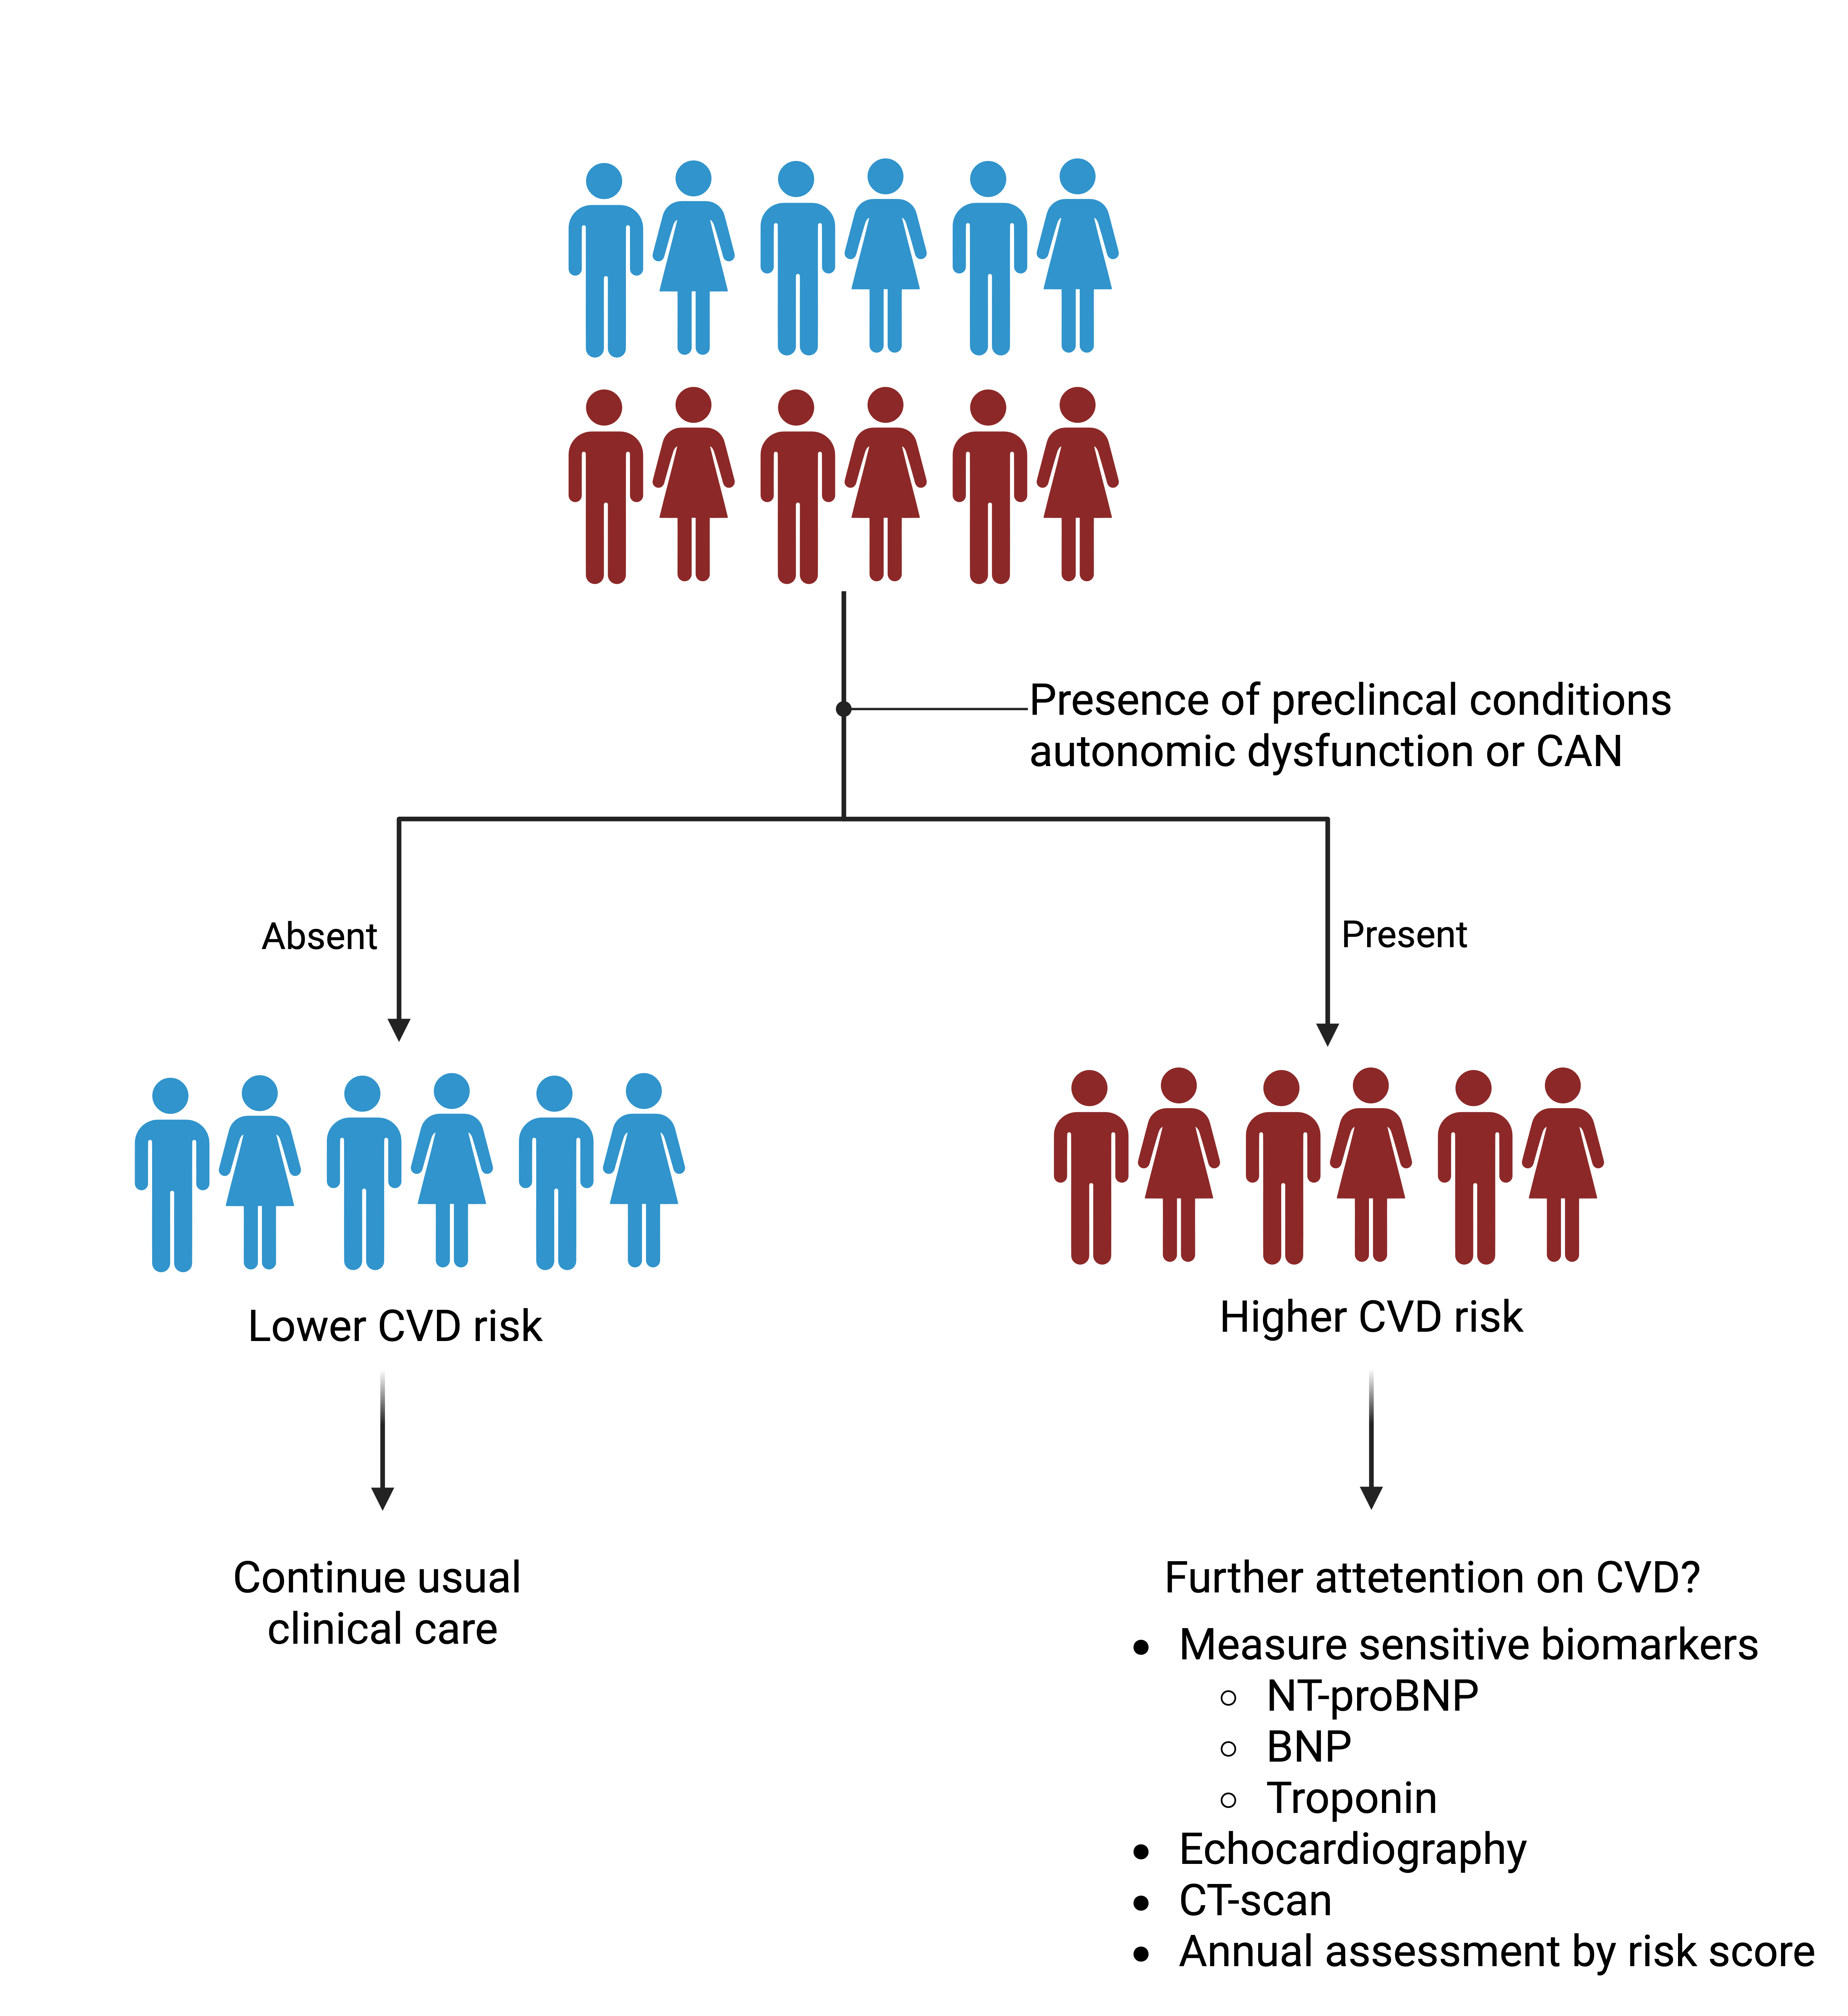
\includegraphics{images/strafication_tree_of_CAN.png}

}

\caption{Risk-stratification by autonomic dysfunction}

}

\end{minipage}%

\end{figure}

\hypertarget{effective-modifiable-marker}{%
\section{Effective modifiable
marker}\label{effective-modifiable-marker}}

\begin{itemize}
\tightlist
\item
  Experimental design of mediation of direct target of HRV (medication:
  beta-blockers, or lifestyle: physical activity and sleep)
\end{itemize}

\begin{figure}

\begin{minipage}[t]{\linewidth}

{\centering 

\raisebox{-\height}{

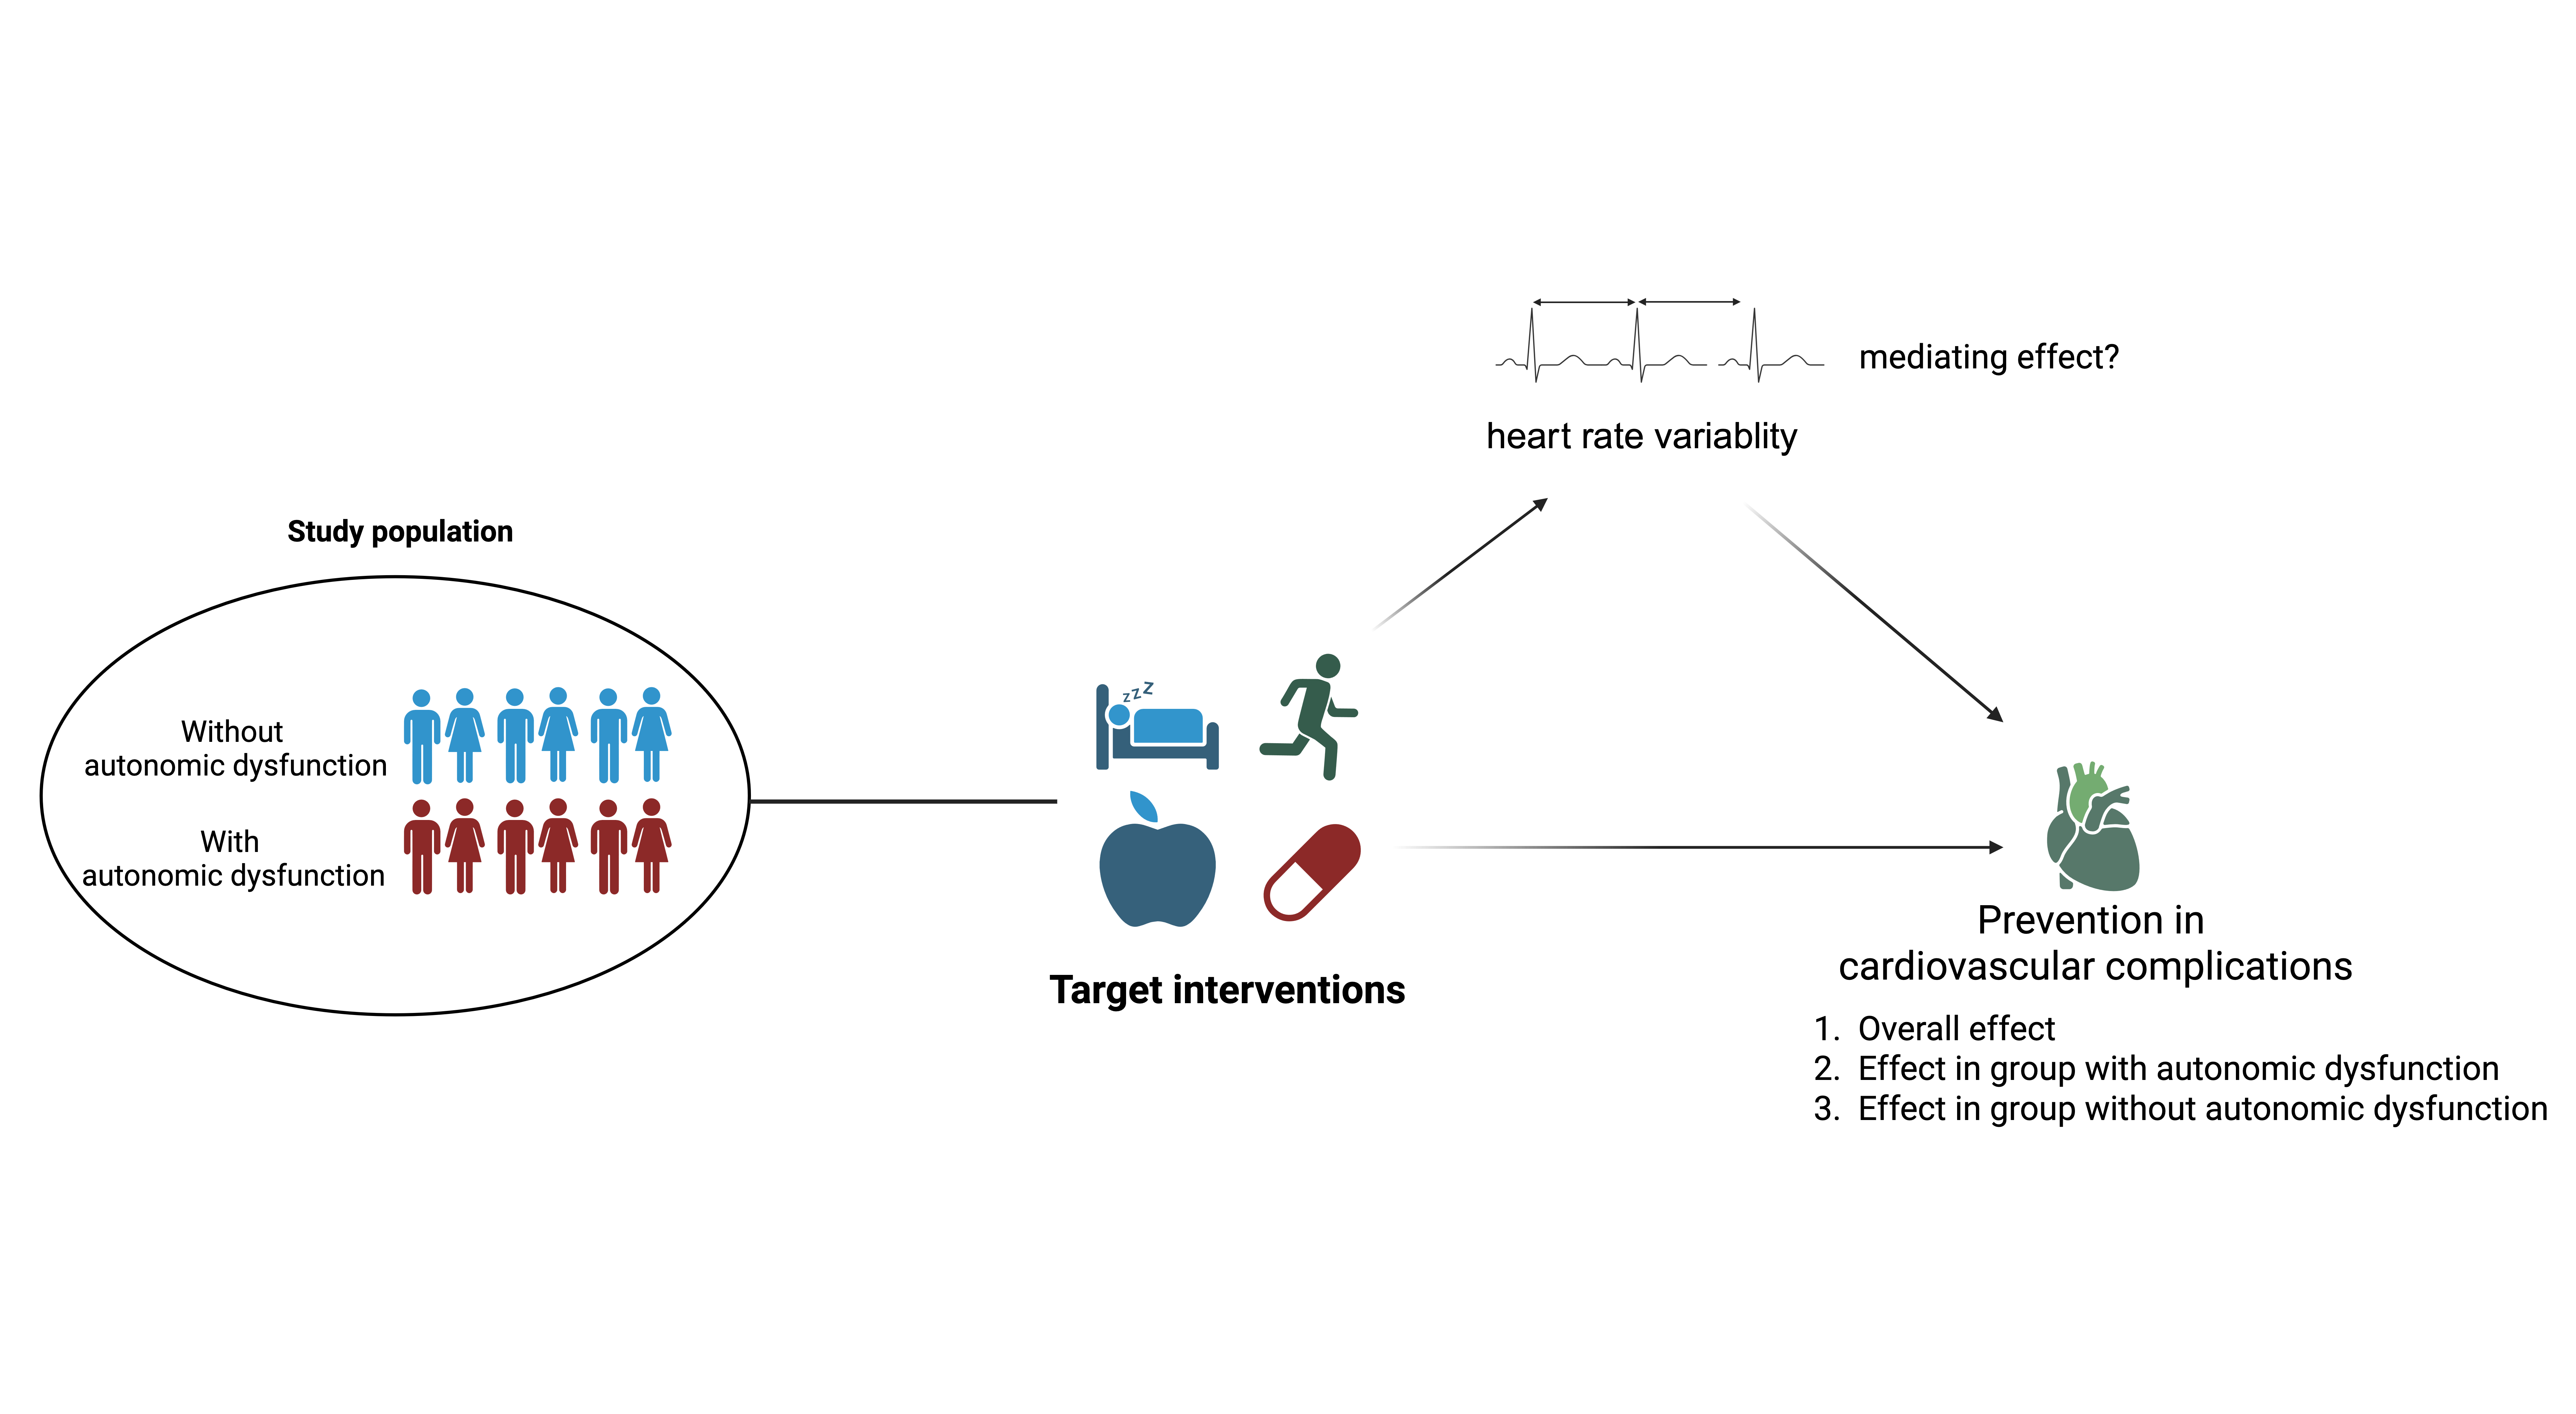
\includegraphics{images/Mediation_HRV.png}

}

\caption{Mediation of HRV by intervention in prevention of CVD}

}

\end{minipage}%

\end{figure}

\bookmarksetup{startatroot}

\hypertarget{conclusion}{%
\chapter{Conclusion}\label{conclusion}}

HRV are linked with CVD risk across glucose metabolism. However, both
diabetes and cardiovascular complication may be a contributor to altered
HRV. As such long-term HRV are proxy for many physiological conditions
both behavioural and pathological. Many measures for cardiovascular
system including cardiovascular autonomic function, arterial stiffness,
NT-proBNP reflects increased risk of CVD and heart failure. Structured
studies are needed to understand their clinical role in CVD prevention.
Either as a target to monitor successfulness of CVD treatment or an
indicator for CVD which lead to stratified decision of further
cardiovascular assessment or treatment.

\bookmarksetup{startatroot}

\hypertarget{references}{%
\chapter*{References}\label{references}}
\addcontentsline{toc}{chapter}{References}

\markboth{References}{References}

\hypertarget{refs}{}
\begin{CSLReferences}{1}{0}
\leavevmode\vadjust pre{\hypertarget{ref-agarwalsunilk.2017}{}}%
Agarwal Sunil K., Norby Faye L., Whitsel Eric A., Soliman Elsayed Z.,
Chen Lin Y., Loehr Laura R., Fuster Valentin, Heiss Gerardo, Coresh
Josef, and Alonso Alvaro. 2017. {``Cardiac Autonomic Dysfunction and
Incidence of Atrial Fibrillation.''} \emph{JACC} 69 (3): 291--99.
\url{https://doi.org/10.1016/j.jacc.2016.10.059}.

\leavevmode\vadjust pre{\hypertarget{ref-arshi2022}{}}%
Arshi, Banafsheh, Sven Geurts, Martijn J. Tilly, Marten van den Berg,
Jan A. Kors, Dimitris Rizopoulos, M. Arfan Ikram, and Maryam Kavousi.
2022. {``Heart Rate Variability Is Associated with Left Ventricular
Systolic, Diastolic Function and Incident Heart Failure in the General
Population.''} \emph{BMC Medicine} 20 (1): 91.
\url{https://doi.org/10.1186/s12916-022-02273-9}.

\leavevmode\vadjust pre{\hypertarget{ref-barr2007}{}}%
Barr, Elizabeth L. M., Paul Z. Zimmet, Timothy A. Welborn, Damien
Jolley, Dianna J. Magliano, David W. Dunstan, Adrian J. Cameron, et al.
2007. {``Risk of Cardiovascular and All-Cause Mortality in Individuals
with Diabetes Mellitus, Impaired Fasting Glucose, and Impaired Glucose
Tolerance.''} \emph{Circulation} 116 (2): 151--57.
\url{https://doi.org/10.1161/CIRCULATIONAHA.106.685628}.

\leavevmode\vadjust pre{\hypertarget{ref-whoneed2012}{}}%
Bendix Carstensen Steno Diabetes Center. 2012. {``Who Needs the Cox
Model Anyway.''} \emph{Stat Med} 31: 10741088.

\leavevmode\vadjust pre{\hypertarget{ref-bentzon2014}{}}%
Bentzon, Jacob Fog, Fumiyuki Otsuka, Renu Virmani, and Erling Falk.
2014. {``Mechanisms of Plaque Formation and Rupture.''}
\emph{Circulation Research} 114 (12): 1852--66.
\url{https://doi.org/10.1161/CIRCRESAHA.114.302721}.

\leavevmode\vadjust pre{\hypertarget{ref-boutouyrie2021}{}}%
Boutouyrie, Pierre, Phil Chowienczyk, Jay D. Humphrey, and Gary F.
Mitchell. 2021. {``Arterial Stiffness and Cardiovascular Risk in
Hypertension.''} \emph{Circulation Research} 128 (7): 864--86.
\url{https://doi.org/10.1161/CIRCRESAHA.121.318061}.

\leavevmode\vadjust pre{\hypertarget{ref-campbell2024}{}}%
Campbell, Patricia, Frans H. Rutten, Matthew My Lee, Nathaniel M.
Hawkins, and Mark C. Petrie. 2024. {``Heart failure with preserved
ejection fraction: everything the clinician needs to know.''}
\emph{Lancet (London, England)} 403 (10431): 1083--92.
\url{https://doi.org/10.1016/S0140-6736(23)02756-3}.

\leavevmode\vadjust pre{\hypertarget{ref-chellappa2025}{}}%
Chellappa, Sarah L., Lei Gao, Jingyi Qian, Nina Vujovic, Peng Li, Kun
Hu, and Frank A. J. L. Scheer. 2025. {``Daytime Eating During Simulated
Night Work~Mitigates Changes in Cardiovascular Risk Factors: Secondary
Analyses of a Randomized Controlled Trial.''} \emph{Nature
Communications} 16 (1): 3186.
\url{https://doi.org/10.1038/s41467-025-57846-y}.

\leavevmode\vadjust pre{\hypertarget{ref-coopmans2020}{}}%
Coopmans, Charlotte, Tan Lai Zhou, Ronald M. A. Henry, Jordi Heijman,
Nicolaas C. Schaper, Annemarie Koster, Miranda T. Schram, et al. 2020.
{``Both Prediabetes and Type 2 Diabetes Are Associated with Lower Heart
Rate Variability: The Maastricht Study.''} \emph{Diabetes Care} 43 (5):
1126--33. \url{https://doi.org/10.2337/dc19-2367}.

\leavevmode\vadjust pre{\hypertarget{ref-cseh2020}{}}%
Cseh, Domonkos, Rachel E. Climie, Lucile Offredo, Catherine Guibout,
Frédérique Thomas, Luca Zanoli, Nicolas Danchin, et al. 2020. {``Type 2
Diabetes Mellitus Is Independently Associated with Decreased Neural
Baroreflex Sensitivity.''} \emph{Arteriosclerosis, Thrombosis, and
Vascular Biology} 40 (5): 1420--28.
\url{https://doi.org/10.1161/ATVBAHA.120.314102}.

\leavevmode\vadjust pre{\hypertarget{ref-donnan2008}{}}%
Donnan, Geoffrey A, Marc Fisher, Malcolm Macleod, and Stephen M Davis.
2008. {``Stroke.''} \emph{The Lancet} 371 (9624): 1612--23.
\url{https://doi.org/10.1016/S0140-6736(08)60694-7}.

\leavevmode\vadjust pre{\hypertarget{ref-gottsuxe4ter2006}{}}%
Gottsäter, Anders, Åsa Rydén Ahlgren, Soumia Taimour, and Göran
Sundkvist. 2006. {``Decreased Heart Rate Variability May Predict the
Progression of Carotid Atherosclerosis in Type 2 Diabetes.''}
\emph{Clinical Autonomic Research} 16 (3): 228--34.
\url{https://doi.org/10.1007/s10286-006-0345-4}.

\leavevmode\vadjust pre{\hypertarget{ref-hadad2021}{}}%
Hadad, Rakin, Bjørn Strøjer Larsen, Philip Weber, Dorte Stavnem, Ole P.
Kristiansen, Olav W. Nielsen, Steen B. Haugaard, and Ahmad Sajadieh.
2021. {``Night-Time Heart Rate Variability Identifies High-Risk People
Among People with Uncomplicated Type 2 Diabetes Mellitus.''}
\emph{Diabetic Medicine} 38 (7): e14559.
\url{https://doi.org/10.1111/dme.14559}.

\leavevmode\vadjust pre{\hypertarget{ref-huggett2003}{}}%
Huggett, Robert J., Eleanor M. Scott, Stephen G. Gilbey, John B. Stoker,
Alan F. Mackintosh, and David A. S. G. Mary. 2003. {``Impact of Type 2
Diabetes Mellitus on Sympathetic Neural Mechanisms in Hypertension.''}
\emph{Circulation} 108 (25): 3097--3101.
\url{https://doi.org/10.1161/01.CIR.0000103123.66264.FE}.

\leavevmode\vadjust pre{\hypertarget{ref-jeffreyj.goldberger2019}{}}%
Jeffrey J. Goldberger, Rishi Arora, Una Buckley, and Kalyanam Shivkumar.
2019. {``Autonomic Nervous System Dysfunction.''} \emph{Journal of the
American College of Cardiology} 73 (10): 1189--1206.
\url{https://doi.org/doi:10.1016/j.jacc.2018.12.064}.

\leavevmode\vadjust pre{\hypertarget{ref-kahn2024}{}}%
Kahn, Steven E., John E. Deanfield, Ole Kleist Jeppesen, Scott S.
Emerson, Trine Welløv Boesgaard, Helen M. Colhoun, Robert F. Kushner, et
al. 2024. {``Effect of Semaglutide on Regression and Progression of
Glycemia in People with Overweight or Obesity but Without Diabetes in
the SELECT Trial.''} \emph{Diabetes Care} 47 (8): 1350--59.
\url{https://doi.org/10.2337/dc24-0491}.

\leavevmode\vadjust pre{\hypertarget{ref-kaze2022}{}}%
Kaze, Arnaud D., Matthew F. Yuyun, Sebhat Erqou, Gregg C. Fonarow, and
Justin B. Echouffo-Tcheugui. 2022. {``Cardiac Autonomic Neuropathy and
Risk of Incident Heart Failure Among Adults with Type 2 Diabetes.''}
\emph{European Journal of Heart Failure} 24 (4): 634--41.
\url{https://doi.org/10.1002/ejhf.2432}.

\leavevmode\vadjust pre{\hypertarget{ref-kenny2019}{}}%
Kenny, Helena C., and E. Dale Abel. 2019. {``Heart Failure in Type 2
Diabetes Mellitus.''} \emph{Circulation Research} 124 (1): 121--41.
\url{https://doi.org/10.1161/CIRCRESAHA.118.311371}.

\leavevmode\vadjust pre{\hypertarget{ref-kumarathurai2016}{}}%
Kumarathurai, Preman, Christian Anholm, Bjørn S. Larsen, Rasmus Huan
Olsen, Sten Madsbad, Ole Kristiansen, Olav W. Nielsen, Steen B.
Haugaard, and Ahmad Sajadieh. 2016. {``Effects of Liraglutide on Heart
Rate and Heart Rate Variability: A Randomized, Double-Blind,
Placebo-Controlled Crossover Study.''} \emph{Diabetes Care} 40 (1):
117--24. \url{https://doi.org/10.2337/dc16-1580}.

\leavevmode\vadjust pre{\hypertarget{ref-lee2012}{}}%
Lee, Meng, Jeffrey L Saver, Keun-Sik Hong, Sarah Song, Kuo-Hsuan Chang,
and Bruce Ovbiagele. 2012. {``Effect of Pre-Diabetes on Future Risk of
Stroke: Meta-Analysis.''} \emph{BMJ : British Medical Journal} 344
(June): e3564. \url{https://doi.org/10.1136/bmj.e3564}.

\leavevmode\vadjust pre{\hypertarget{ref-li2024}{}}%
Li, Xin-yu, Xiang-meng Kong, Cheng-hao Yang, Zhi-feng Cheng, Jia-jie Lv,
Hong Guo, and Xiao-hong Liu. 2024. {``Global, Regional, and National
Burden of Ischemic Stroke, 1990{\textendash}2021: An Analysis of Data
from the Global Burden of Disease Study 2021.''}
\emph{eClinicalMedicine} 75 (September).
\url{https://doi.org/10.1016/j.eclinm.2024.102758}.

\leavevmode\vadjust pre{\hypertarget{ref-lu2023}{}}%
Lu, Y., S. J. Kiechl, J. Wang, Q. Xu, S. Kiechl, and R. Pechlaner. 2023.
{``Global distributions of age- and sex-related arterial stiffness:
systematic review and meta-analysis of 167 studies with 509,743
participants.''} \emph{EBioMedicine} 92 (June): 104619.
\url{https://doi.org/10.1016/j.ebiom.2023.104619}.

\leavevmode\vadjust pre{\hypertarget{ref-mceniery2017}{}}%
McEniery, Carmel M., Ian B. Wilkinson, Nanna B. Johansen, Daniel R.
Witte, Archana Singh-Manoux, Mika Kivimaki, Adam G. Tabak, Eric J.
Brunner, and Martin J. Shipley. 2017. {``Nondiabetic Glucometabolic
Status and Progression of Aortic Stiffness: The Whitehall II Study.''}
\emph{Diabetes Care} 40 (4): 599--606.
\url{https://doi.org/10.2337/dc16-1773}.

\leavevmode\vadjust pre{\hypertarget{ref-mohanta2022}{}}%
Mohanta, Sarajo K., Li Peng, Yuanfang Li, Shu Lu, Ting Sun, Lorenzo
Carnevale, Marialuisa Perrotta, et al. 2022. {``Neuroimmune
Cardiovascular Interfaces Control Atherosclerosis.''} \emph{Nature} 605
(7908): 152--59. \url{https://doi.org/10.1038/s41586-022-04673-6}.

\leavevmode\vadjust pre{\hypertarget{ref-niemeluxe41994}{}}%
Niemelä, M. J., K. E. Airaksinen, and H. V. Huikuri. 1994. {``Effect of
beta-blockade on heart rate variability in patients with coronary artery
disease.''} \emph{Journal of the American College of Cardiology} 23 (6):
1370--77. \url{https://doi.org/10.1016/0735-1097(94)90379-4}.

\leavevmode\vadjust pre{\hypertarget{ref-normand2019}{}}%
Normand, Camilla, David M Kaye, Thomas J Povsic, and Kenneth Dickstein.
2019. {``Beyond Pharmacological Treatment: An Insight into Therapies
That Target Specific Aspects of Heart Failure Pathophysiology.''}
\emph{The Lancet} 393 (10175): 1045--55.
\url{https://doi.org/10.1016/S0140-6736(18)32216-5}.

\leavevmode\vadjust pre{\hypertarget{ref-osei2024}{}}%
Osei, Jeffery, Viola Vaccarino, Maggie Wang, Anish S. Shah, Rachel
Lampert, Louis Y. Li, Yi-An Ko, et al. 2024. {``Stress-Induced Autonomic
Dysfunction Is Associated with Mental Stress{\textendash}induced
Myocardial Ischemia in Patients with Coronary Artery Disease.''}
\emph{Circulation: Cardiovascular Imaging} 17 (6): e016596.
\url{https://doi.org/10.1161/CIRCIMAGING.124.016596}.

\leavevmode\vadjust pre{\hypertarget{ref-picard2021}{}}%
Picard, Mathilde, Igor Tauveron, Salwan Magdasy, Thomas Benichou, Reza
Bagheri, Ukadike C. Ugbolue, Valentin Navel, and Frédéric Dutheil. 2021.
{``Effect of Exercise Training on Heart Rate Variability in Type 2
Diabetes Mellitus Patients: A Systematic Review and Meta-Analysis.''}
\emph{PLOS ONE} 16 (5): e0251863.
\url{https://doi.org/10.1371/journal.pone.0251863}.

\leavevmode\vadjust pre{\hypertarget{ref-vanpopele2001}{}}%
Popele, Nicole M. van, Diederick E. Grobbee, Michiel L. Bots, Roland
Asmar, Jirar Topouchian, Robert S. Reneman, Arnold P. G. Hoeks, Deidre
A. M. van der Kuip, Albert Hofman, and Jacqueline C. M. Witteman. 2001.
{``Association Between Arterial Stiffness and Atherosclerosis.''}
\emph{Stroke} 32 (2): 454--60.
\url{https://doi.org/10.1161/01.STR.32.2.454}.

\leavevmode\vadjust pre{\hypertarget{ref-reductio2002}{}}%
{``Reduction in the Incidence of Type 2 Diabetes with Lifestyle
Intervention or Metformin.''} 2002. \emph{New England Journal of
Medicine} 346 (6): 393--403. \url{https://doi.org/10.1056/NEJMoa012512}.

\leavevmode\vadjust pre{\hypertarget{ref-rinaldi2023}{}}%
Rinaldi, Elisabetta, Frank C. T. van der Heide, Enzo Bonora, Maddalena
Trombetta, Chiara Zusi, Abraham A. Kroon, Miranda T. Schram, et al.
2023. {``Lower Heart Rate Variability, an Index of Worse Autonomic
Function, Is Associated with Worse Beta Cell Response to a Glycemic Load
in Vivo{\textemdash}the Maastricht Study.''} \emph{Cardiovascular
Diabetology} 22 (1): 105.
\url{https://doi.org/10.1186/s12933-023-01837-0}.

\leavevmode\vadjust pre{\hypertarget{ref-schaarup2024a}{}}%
Schaarup, Jonas. 2024. {``Actiheart Validation of Time-Domain Heart Rate
Variability.''}
\url{https://figshare.com/articles/online_resource/Actiheart_validation_of_time-domain_heart_rate_variability/26182361}.

\leavevmode\vadjust pre{\hypertarget{ref-schaarup2023}{}}%
Schaarup, Jonas R., Martin S. Christensen, Adam Hulman, Christian S.
Hansen, Dorte Vistisen, Adam G. Tabák, Daniel R. Witte, and Lasse Bjerg.
2023. {``Autonomic Dysfunction Is Associated with the Development of
Arterial Stiffness: The Whitehall II Cohort.''} \emph{GeroScience} 45
(4): 2443--55. \url{https://doi.org/10.1007/s11357-023-00762-0}.

\leavevmode\vadjust pre{\hypertarget{ref-schlaich2015}{}}%
Schlaich, M., N. Straznicky, E. Lambert, and G. Lambert. 2015.
{``Metabolic syndrome: a sympathetic disease?''} \emph{Lancet Diabetes
Endocrinol} 3 (2): 148--57.
\url{https://doi.org/10.1016/s2213-8587(14)70033-6}.

\leavevmode\vadjust pre{\hypertarget{ref-shah2015}{}}%
Shah, Anoop Dinesh, Claudia Langenberg, Eleni Rapsomaniki, Spiros
Denaxas, Mar Pujades-Rodriguez, Chris P Gale, John Deanfield, Liam
Smeeth, Adam Timmis, and Harry Hemingway. 2015. {``Type 2 Diabetes and
Incidence of Cardiovascular Diseases: A Cohort Study in 1·9 Million
People.''} \emph{The Lancet Diabetes \& Endocrinology} 3 (2): 105--13.
\url{https://doi.org/10.1016/S2213-8587(14)70219-0}.

\leavevmode\vadjust pre{\hypertarget{ref-shen2014}{}}%
Shen, Mark J., and Douglas P. Zipes. 2014. {``Role of the Autonomic
Nervous System in Modulating Cardiac Arrhythmias.''} \emph{Circulation
Research} 114 (6): 1004--21.
\url{https://doi.org/10.1161/CIRCRESAHA.113.302549}.

\leavevmode\vadjust pre{\hypertarget{ref-vos2020}{}}%
Vos, Theo, Stephen S Lim, Cristiana Abbafati, Kaja M Abbas, Mohammad
Abbasi, Mitra Abbasifard, Mohsen Abbasi-Kangevari, et al. 2020.
{``Global Burden of 369 Diseases and Injuries in 204 Countries and
Territories, 1990{\textendash}2019: A Systematic Analysis for the Global
Burden of Disease Study 2019.''} \emph{The Lancet} 396 (10258):
1204--22. \url{https://doi.org/10.1016/S0140-6736(20)30925-9}.

\leavevmode\vadjust pre{\hypertarget{ref-yusuf2020}{}}%
Yusuf, Salim, Philip Joseph, Sumathy Rangarajan, Shofiqul Islam, Andrew
Mente, Perry Hystad, Michael Brauer, et al. 2020. {``Modifiable Risk
Factors, Cardiovascular Disease, and Mortality in 155{\hphantom{,}}722
Individuals from 21 High-Income, Middle-Income, and Low-Income Countries
(PURE): A Prospective Cohort Study.''} \emph{The Lancet} 395 (10226):
795--808. \url{https://doi.org/10.1016/S0140-6736(19)32008-2}.

\leavevmode\vadjust pre{\hypertarget{ref-zaman}{}}%
Zaman, Sarah, Jason H Wasfy, Vikas Kapil, Boback Ziaeian, William A
Parsonage, Sira Sriswasdi, Timothy J A Chico, et al. n.d. {``The Lancet
Commission on Rethinking Coronary Artery Disease: Moving from Ischaemia
to Atheroma.''} \emph{The Lancet}.
\url{https://doi.org/10.1016/S0140-6736(25)00055-8}.

\end{CSLReferences}

\cleardoublepage
\phantomsection
\addcontentsline{toc}{part}{Appendices}
\appendix

\hypertarget{sec-more-results}{%
\chapter{More results}\label{sec-more-results}}

Some results that wouldn't fit into the main thesis

\hypertarget{another-appendix}{%
\chapter{Another appendix}\label{another-appendix}}

Something else


\backmatter

\end{document}
